\documentclass[a4paper,12pt]{article}
\usepackage[utf8]{inputenc}
\usepackage[ngerman]{babel}
\usepackage{amsmath}
\usepackage{amssymb}
\usepackage{amsthm}
\usepackage{geometry}
\usepackage{graphicx}
\usepackage[hidelinks]{hyperref}
\usepackage{listings}
\usepackage{xcolor}
\usepackage{algorithm}
\usepackage{algpseudocode}
\usepackage{chngcntr}
\usepackage{booktabs}
\usepackage{enumitem}
\setlist[itemize]{label=-}

\geometry{margin=2.5cm}

% Code-Highlighting
\lstset{
	basicstyle=\ttfamily\small,
	keywordstyle=\color{blue},
	commentstyle=\color{gray},
	stringstyle=\color{red},
	numbers=left,
	numberstyle=\tiny,
	breaklines=true,
	frame=single
}

\theoremstyle{definition}
\newtheorem{definition}{Definition}[section]
\newtheorem{beispiel}{Beispiel}[section]
\newtheorem{theorem}{Theorem}[section]
\newtheorem{satz}{Satz}[section]
\newtheorem{lemma}{Lemma}[section]
\newtheorem{example}{Beispiel}[section]
\newtheorem{remark}{Bemerkung}[section]
\newtheorem{kreuzung}{Kreuzung}[section]
\newtheorem{potential}{Forschungspotential}[section]

\title{Model Checking $\times$ Roboternavigation\\
	\large{Formale Verifikation autonomer Phi-basierter Navigationssysteme}}

\author{Stephan Epp}

\date{\today}
\usepackage[protrusion=true,expansion=false]{microtype}
\usepackage{float}
\usepackage{tikz}
\usetikzlibrary{positioning, shapes, arrows.meta, shadows}

% Verhindere Textüberlauf über den rechten DIN A4 Rand
\sloppy
\emergencystretch=3em
\setlength{\hfuzz}{2pt}

\begin{document}


	
\maketitle

\tableofcontents
\newpage

\section{Einleitung}

Diese Arbeit präsentiert die systematische Kreuzung zweier wissenschaftlicher Arbeiten: \textit{Model Checking mit dem Subgraph Algorithmus} und \textit{Phi-Navigation für Roboter}. Durch die Kombination der formalen Verifikationstechniken des Model Checkings mit der biologisch inspirierten Phi-Navigation entstehen neue Forschungspotentiale für verifizierte autonome Robotersysteme. Wir identifizieren konkrete Synergien, entwickeln einen formalen Rahmen für die Verifikation von Navigationssystemen und präsentieren ein Vorgehen zur Integration von temporaler Logik (CTL/LTL) mit $\phi$-exponentiellen Potentialfeldern. Die Arbeit zeigt, wie graphbasierte Model-Checking-Algorithmen mit polynomialer Laufzeit $O(n^3)$ zur Verifikation von Navigationseigenschaften eingesetzt werden können und wie sich die natürliche Robustheit der Phi-Navigation formal beweisen lässt.

\subsection{Motivation}

Die autonome Roboternavigation steht vor zwei fundamentalen Herausforderungen:

\begin{enumerate}
	\item \textbf{Effizienz und Natürlichkeit}: Klassische Planungsalgorithmen (A*, RRT, Dijkstra) erfordern globale Kartierung und umfangreiche Berechnungen. Die Phi-Navigation bietet ein biologisch inspiriertes, lokal operierendes Vorgehen mit minimaler Energiedissipation.
	
	\item \textbf{Sicherheit und Verifizierbarkeit}: Autonome Systeme müssen sicherheitskritische Eigenschaften garantieren (Kollisionsfreiheit, Zielerreichung, Liveness). Model Checking ermöglicht formale Verifikation dieser Eigenschaften.
\end{enumerate}

Die Kreuzung dieser beiden Ansätze eröffnet ein neues Forschungsfeld: \textbf{formal verifizierte, biologisch inspirierte Roboternavigation}.

\subsection{Die beiden Quellarbeiten}

\subsubsection{Model Checking mit Subgraph Algorithmus}

Diese Arbeit entwickelt eine graphbasierte Vorgehensweise zur formalen Verifikation mit folgenden Kernbeiträgen:

\begin{itemize}
	\item \textbf{Subgraph Algorithmus}: Polynomiale Signaturen für effiziente Subgraph-Bezie\-hungsprüfung
	\item \textbf{Komplexität}: $O(n^3)$ für Subgraph-Matching (vs. $O(n!)$ für klassische Algorithmen)
	\item \textbf{Temporale Logik}: Algorithmen für LTL (Linear Temporal Logic) und CTL (Computation Tree Logic)
	\item \textbf{Kripke-Strukturen}: Graphbasierte Repräsentation von Systemzuständen
	\item \textbf{Verifikation}: Safety-, Liveness- und Reachability-Properties
\end{itemize}

\subsubsection{Phi-Navigation für Roboter}

Diese Arbeit präsentiert eine neuartige Navigationsmethode basierend auf dem goldenen Schnitt $\phi = \frac{1+\sqrt{5}}{2} \approx 1{,}618$:

\begin{itemize}
	\item \textbf{Lokales Prinzip}: Navigation nur mit lokalen Sensorinformationen
	\item \textbf{$\phi$-Exponentialfunktion}: Geschwindigkeitsprofil $v(d) = v_{\max}(1 - e^{-\phi d/d_{\text{ref}}})$
	\item \textbf{Energieoptimalität}: Minimale Energiedissipation durch $\phi$-Parameter
	\item \textbf{Robustheit}: Anpassung an Umgebungsänderungen ohne globale Neuplanung
	\item \textbf{Bio-Inspiration}: Orientierung an natürlichen Navigationssystemen (Bienen)
\end{itemize}

\subsection{Forschungsfragen der Kreuzung}

Die Integration dieser beiden Ansätze wirft folgende zentrale Fragen auf:

\begin{enumerate}
	\item Wie lassen sich Navigationseigenschaften der Phi-Navigation formal in temporaler Logik spezifizieren?
	\item Kann der Subgraph Algorithmus effizient zur Verifikation von Navigationssystemen eingesetzt werden?
	\item Welche Garantien können für $\phi$-basierte Navigation formal bewiesen werden?
	\item Wie können Kripke-Strukturen für kontinuierliche Navigationssysteme konstruiert werden?
	\item Welche neuen Verifikationstechniken entstehen aus der Kombination?
\end{enumerate}

\subsection{Beiträge dieser Arbeit}

Diese Kreuzungsanalyse liefert folgende wissenschaftliche Beiträge:

\begin{enumerate}
	\item \textbf{Formaler Rahmen}: Integration von Model Checking und Phi-Navigation
	\item \textbf{Verifikationsalgorithmen}: Anpassung des Subgraph Algorithmus für Navigationssysteme
	\item \textbf{Spezifikationssprache}: CTL/LTL-Formeln für Navigationseigenschaften
	\item \textbf{Theoretische Garantien}: Formale Beweise für Safety und Liveness
	\item \textbf{Forschungspotentiale}: Identifikation von 10 konkreten Forschungsrichtungen
\end{enumerate}


\section{Property Pattern Graph: Annäherung an das Ziel}\label{sec:tikz}

Das folgende TikZ-Diagramm aus der zugehörigen Beweisarbeit visualisiert den Property Pattern Graph für die monotone Annäherung an das Ziel in der Phi-Navigation (vgl.~Abschnitt~\ref{app:beweise}).

\begin{figure}[h]
\centering
\begin{tikzpicture}[
    node distance=2.5cm,
    state/.style={
        rectangle,
        rounded corners=5pt,
        draw=blue!70,
        fill=blue!10,
        very thick,
        minimum width=6cm,
        minimum height=1.5cm,
        align=center,
        font=\small\sffamily,
        drop shadow
    },
    arrow/.style={
        -Stealth,
        very thick,
        blue!70,
        shorten >=2pt,
        shorten <=2pt
    },
    label/.style={
        font=\scriptsize\ttfamily,
        blue!80
    }
]

% State 1
\node[state] (s1) {
    \textbf{State 1}\\[0.1cm]
    \texttt{far\_from\_goal}\\
    \texttt{high\_velocity}
};

% State 2
\node[state, below=of s1] (s2) {
    \textbf{State 2}\\[0.1cm]
    \texttt{medium\_distance}\\
    \texttt{medium\_velocity}
};

% State 3
\node[state, below=of s2] (s3) {
    \textbf{State 3}\\[0.1cm]
    \texttt{close\_to\_goal}\\
    \texttt{low\_velocity}
};

% State 4
\node[state, below=of s3, fill=green!10, draw=green!70] (s4) {
    \textbf{State 4}\\[0.1cm]
    \texttt{at\_goal}\\
    \texttt{zero\_velocity}
};

% Arrows
\draw[arrow] (s1) -- (s2);
\draw[arrow] (s2) -- (s3);
\draw[arrow] (s3) -- (s4);

% Distance annotations (right side)
\node[right=1.5cm of s1, label] {$d \gg d_{\text{ref}}$};
\node[right=1.5cm of s2, label] {$d \approx d_{\text{ref}}$};
\node[right=1.5cm of s3, label] {$d \ll d_{\text{ref}}$};
\node[right=1.5cm of s4, label] {$d \leq \epsilon$};

\end{tikzpicture}
\caption{Property Pattern Graph für monotone Annäherung an das Ziel. Die vier Zustände repräsentieren charakteristische Phasen der Phi-Navigation: weit vom Ziel entfernt mit hoher Geschwindigkeit, mittlere Distanz mit mittlerer Geschwindigkeit, nahe am Ziel mit niedriger Geschwindigkeit und schließlich am Ziel mit Stillstand. Die rechte Seite zeigt die zugehörigen Distanzen relativ zur Referenzdistanz $d_{\text{ref}}$.}
\label{fig:pattern}
\end{figure}

\section{Formaler Rahmen}

\subsection{Kripke-Struktur für Phi-Navigation}

\begin{definition}[Navigations-Kripke-Struktur]
Eine Navigations-Kripke-Struktur für ein Phi-basiertes Robotersystem ist ein 6-Tupel
\[
\mathcal{K}_{\phi} = (S, S_0, R, AP, L, \phi)
\]
wobei:
\begin{itemize}
	\item $S$: Endliche Menge von Zuständen (diskretisierte Positionen $\times$ Geschwindigkeiten)
	\item $S_0 \subseteq S$: Menge der Initialzustände
	\item $R \subseteq S \times S$: Transitionsrelation gemäß Phi-Navigationsdynamik
	\item $AP$: Menge atomarer Propositionen (z.B. \texttt{at\_goal}, \texttt{collision\_free}, \texttt{moving})
	\item $L: S \to 2^{AP}$: Labeling-Funktion
	\item $\phi = \frac{1+\sqrt{5}}{2}$: Goldener Schnitt als Systemparameter
\end{itemize}
\end{definition}

\begin{beispiel}[Diskretisierung des Zustandsraums]
Für einen 2D-Roboter mit Arbeitsraum $[0,10] \times [0,10]$ und Geschwindigkeitsbereich $[0, v_{\max}]$:
\begin{itemize}
	\item Räumliche Diskretisierung: $100 \times 100$ Grid ($\Delta x = \Delta y = 0{,}1$)
	\item Geschwindigkeitsdiskretisierung: 10 Stufen
	\item Gesamtzahl Zustände: $|S| = 100 \times 100 \times 10 = 100{,}000$
\end{itemize}

Atomare Propositionen:
\begin{itemize}
	\item $\texttt{at\_goal}$: Position innerhalb $\epsilon$-Umgebung des Ziels
	\item $\texttt{collision\_free}$: Keine Ãœberlappung mit Hindernissen
	\item $\texttt{low\_velocity}$: $v < 0{,}2 \cdot v_{\max}$
	\item $\texttt{approaching}$: Distanz zum Ziel nimmt ab
\end{itemize}
\end{beispiel}

\subsection{Transitionsrelation durch Phi-Dynamik}

Die Transitionsrelation $R$ wird durch die $\phi$-exponentielle Geschwindigkeitsfunktion bestimmt:

\begin{definition}[Phi-Transition]
Zwei Zustände $s = (x, y, v)$ und $s' = (x', y', v')$ stehen in Relation $s \xrightarrow{\phi} s'$ genau dann, wenn:
\[
\begin{cases}
x' = x + v \cdot \Delta t \cdot \cos(\theta) \\
y' = y + v \cdot \Delta t \cdot \sin(\theta) \\
v' = v_{\max}(1 - e^{-\phi d(s)/d_{\text{ref}}}) \\
\theta = \text{atan2}(y_{\text{goal}} - y, x_{\text{goal}} - x)
\end{cases}
\]
wobei $d(s)$ die Distanz vom Zustand $s$ zum Ziel und $\Delta t$ der Zeitschritt ist.
\end{definition}

\begin{lemma}[Determinismus der Phi-Navigation]
Für feste Parameter $v_{\max}, d_{\text{ref}}, \Delta t$ ist die Transitionsrelation $R$ deterministisch: Für jeden Zustand $s$ existiert höchstens ein Nachfolgezustand $s'$ mit $s \xrightarrow{\phi} s'$.
\end{lemma}

\begin{proof}
Die Transition ist durch die Formeln für $(x', y', v')$ eindeutig bestimmt. Die Richtung $\theta$ ergibt sich eindeutig aus der aktuellen Position und dem festen Ziel. Die neue Geschwindigkeit $v'$ ist eine deterministische Funktion der aktuellen Distanz. Somit ist $s'$ eindeutig.
\end{proof}

\subsection{Temporale Eigenschaften der Phi-Navigation}

Wir spezifizieren zentrale Navigationseigenschaften in CTL und LTL:

\subsubsection{Safety-Properties}

\begin{satz}[Kollisionsfreiheit in CTL]
Die Kollisionsfreiheit kann ausgedrückt werden als:
\[
\text{AG}(\texttt{collision\_free})
\]
Dies bedeutet: Auf allen Pfaden gilt zu allen Zeitpunkten, dass keine Kollision vorliegt.
\end{satz}

\begin{satz}[Geschwindigkeitsbeschränkung]
Die Einhaltung der Maximalgeschwindigkeit:
\[
\text{AG}(v \leq v_{\max})
\]
\end{satz}

\subsubsection{Liveness-Properties}

\begin{satz}[Eventuelle Zielerreichung in CTL]
Unter der Annahme kollisionsfreier Pfade gilt:
\[
\text{AF}(\texttt{at\_goal})
\]
Dies garantiert: Auf allen Pfaden wird schließlich das Ziel erreicht.
\end{satz}

\begin{satz}[Monotoner Fortschritt in LTL]
Der Roboter nähert sich dem Ziel monoton:
\[
\text{G}(\texttt{approaching} \lor \texttt{at\_goal})
\]
\end{satz}

\subsubsection{Fairness-Properties}

\begin{satz}[Faire Bewegung]
Der Roboter ist nicht permanent stillstehend:
\[
\text{GF}(\neg \texttt{low\_velocity})
\]
\end{satz}

\section{Verifikation mit dem Subgraph Algorithmus}

\subsection{Anwendung auf Navigationssysteme}

Der Subgraph Algorithmus kann zur effizienten Verifikation von Navigationseigenschaften eingesetzt werden:

\begin{definition}[Property Pattern Graph]
Ein Property Pattern Graph $G_P = (V_P, E_P)$ ist ein gerichteter Graph, der ein gewünschtes Verhaltensmuster kodiert:
\begin{itemize}
	\item Knoten $V_P$ repräsentieren Zustände mit bestimmten Eigenschaften
	\item Kanten $E_P$ repräsentieren erlaubte/geforderte Transitionen
\end{itemize}
\end{definition}

\begin{beispiel}[Pattern Annäherung-an-Ziel] Das Pattern für Annäherung an Ziel:
\begin{verbatim}
State 1: far_from_goal, high_velocity
    |
    v
State 2: medium_distance, medium_velocity
    |
    v
State 3: close_to_goal, low_velocity
    |
    v
State 4: at_goal, zero_velocity
\end{verbatim}

Dieses Pattern kann als Subgraph $G_P$ mit 4 Knoten dargestellt werden. Die Verifikation prüft, ob $G_P$ ein Subgraph der Navigations-Kripke-Struktur $\mathcal{K}_{\phi}$ ist.
\end{beispiel}

\subsection{Signatur-basierte Verifikation}

Der Subgraph Algorithmus nutzt Signaturen für effiziente Verifikation:

\begin{algorithm}
\caption{Verify Navigation Property}
\begin{algorithmic}[1]
\State \textbf{Input:} Kripke-Struktur $\mathcal{K}_{\phi}$, Property Pattern $G_P$
\State \textbf{Output:} True falls Property erfüllt, False sonst
\State 
\State Konvertiere $\mathcal{K}_{\phi}$ zu Adjazenzmatrix $A$
\State Konvertiere $G_P$ zu Adjazenzmatrix $B$
\State 
\State \textbf{// Berechne Signaturen}
\For{$j = 0$ to $n_A - 1$}
    \State $\sigma_j^A = \sum_{i=0}^{n_A-1} A_{ij} \cdot 2^i + j \cdot 2^{n_A}$
\EndFor
\For{$j = 0$ to $n_B - 1$}
    \State $\sigma_j^B = \sum_{i=0}^{n_B-1} B_{ij} \cdot 2^i + j \cdot 2^{n_B}$
\EndFor
\State 
\State \textbf{// Teste zyklische Rotationen}
\For{$k = 0$ to $n_B - 1$}
    \State Rotiere $\text{Sig}_B$ um $k$ Positionen
    \If{Rotiertes $\text{Sig}_B$ in $\text{Sig}_A$ enthalten}
        \State \Return True
    \EndIf
\EndFor
\State \Return False
\end{algorithmic}
\end{algorithm}

\begin{theorem}[Korrektheit der Verifikation]
Der Algorithmus liefert genau dann True, wenn das Property Pattern $G_P$ als Subgraph in der Navigations-Kripke-Struktur existiert.
\end{theorem}

\begin{proof}
Die Korrektheit folgt aus der Injektivität der Signatur-Funktion (siehe Lemma in mc.tex). Ein Match der Signaturen impliziert strukturelle Übereinstimmung der Graphen, was wiederum die Existenz des Verhaltensmusters garantiert.
\end{proof}

\subsection{Komplexitätsanalyse}

\begin{theorem}[Laufzeit der Verifikation]
Die Verifikation eines Property Patterns mit $m$ Zuständen in einer Navigations-Kripke-Struktur mit $n$ Zuständen hat Laufzeit:
\[
T(n,m) = O(n^2 + m \cdot n) = O(n^2)
\]
für $m \ll n$.
\end{theorem}

\begin{proof}
\begin{itemize}
	\item Signaturberechnung für $\mathcal{K}_{\phi}$: $O(n^2)$ (für jeden der $n$ Knoten werden $n$ Einträge summiert)
	\item Signaturberechnung für $G_P$: $O(m^2)$
	\item Rotation und Matching: $O(m \cdot n)$ (für jede der $m$ Rotationen Vergleich mit $n$ Signaturen)
	\item Gesamt: $O(n^2 + m^2 + m \cdot n) = O(n^2)$ für $m = O(\sqrt{n})$
\end{itemize}
\end{proof}

Dies ist eine dramatische Verbesserung gegenüber klassischem Model Checking mit exponentieller Komplexität $O(2^n)$.

\section{Theoretische Garantien der Phi-Navigation}

\subsection{Formaler Beweis der Zielerreichung}

\begin{theorem}[Garantierte Zielerreichung]
Sei $\mathcal{K}_{\phi}$ eine Navigations-Kripke-Struktur für hindernisfreien Raum. Dann gilt:
\[
\mathcal{K}_{\phi} \models \text{AF}(\texttt{at\_goal})
\]
\end{theorem}

\begin{proof}
Wir zeigen, dass jeder Pfad schließlich das Ziel erreicht:

\textbf{Lyapunov-Funktion}: Betrachte die Distanzfunktion $V(s) = d(s)$ vom Zustand $s$ zum Ziel.

\textbf{Monotonie}: Nach Definition der Phi-Transition gilt:
\[
V(s') < V(s) \quad \text{für alle } s \xrightarrow{\phi} s' \text{ mit } V(s) > \epsilon
\]
wobei $\epsilon$ die Zieltoleranz ist. Dies folgt, da die Bewegungsrichtung stets zum Ziel zeigt.

\textbf{Beschränktheit}: $V(s) \geq 0$ für alle $s$, und $V(s) = 0$ genau dann, wenn $s \models \texttt{at\_goal}$.

\textbf{Konvergenz}: Da $V$ monoton fällt und nach unten beschränkt ist, konvergiert jeder Pfad gegen einen Zustand mit $V(s) \leq \epsilon$, also $\texttt{at\_goal}$.

Somit gilt $\text{AF}(\texttt{at\_goal})$ für alle Initialzustände.
\end{proof}

\subsection{Formaler Beweis der Energieoptimalität}

\begin{theorem}[Minimale Energiedissipation]
Das $\phi$-exponentielle Geschwindigkeitsprofil minimiert die Energiedissipation unter allen Profilen, die das Ziel in vorgegebener Zeit erreichen.
\end{theorem}

\begin{proof}[Beweisskizze]
Die Gesamtenergie ist:
\[
E = \int_0^T P(t) \, dt = \int_0^T F \cdot v(t) \, dt
\]

Für das $\phi$-Profil $v(t) = v_{\max}(1 - e^{-\phi t/\tau})$ gilt:
\[
E_{\phi} = \int_0^T F \cdot v_{\max}(1 - e^{-\phi t/\tau}) \, dt
\]

Die Variationsrechnung zeigt (vgl. \cite{phi_energy}), dass $\phi$ der Exponent ist, der $E_{\phi}$ minimiert unter der Nebenbedingung konstanter Durchschnittsgeschwindigkeit.
\end{proof}

\subsection{Robustheit gegenüber Umgebungsänderungen}

\begin{theorem}[Robustheit]
Die Phi-Navigation ist robust gegenüber dynamischen Hindernissen: Wenn ein Hindernis während der Navigation erscheint, passt sich der Roboter lokal an, ohne globale Neuplanung.
\end{theorem}

\begin{proof}
Die Phi-Navigation basiert ausschließlich auf aktuellen lokalen Sensordaten. Än\-derungen in der Umgebung:
\begin{itemize}
	\item Werden sofort durch Sensoren erkannt
	\item Führen zu lokaler Anpassung der Richtung $\theta$
	\item Erfordern keine Änderung globaler Pläne (da keine existieren)
\end{itemize}
Die Konvergenzeigenschaften (Theorem 4.1) bleiben erhalten, solange ein kollisionsfreier Pfad existiert.
\end{proof}

\section{Integration: Verifizierte Phi-Navigation}

\subsection{Architektur eines verifizierten Navigationssystems}

Das Architekturdiagramm visualisiert ein vollständiges, mehrschichtiges System für formal verifizierte autonome Roboternavigation, das auf dem goldenen Schnitt $\phi$ basiert. Die Architektur ist als vertikaler Datenfluss konzipiert, bei dem Informationen von oben nach unten durch vier klar abgegrenzte Komponenten fließen. Jede Komponente erfüllt eine spezifische Funktion im Gesamtsystem und kommuniziert mit den benachbarten Schichten durch wohldefinierte Schnittstellen. Die hierarchische Anordnung spiegelt sowohl den zeitlichen Ablauf der Verarbeitung als auch die zunehmende Abstraktion wider: von konkreten physikalischen Sensordaten über mathematische Modellierung bis hin zu abstrakten Verifikationsresultaten und schließlich Sicherheitsüberwachung.

Abbildung \ref{fig:arch} zeigt den Aufbau der Architektur des verifizierten Navigationssystems für die Phi-Navigation.

\begin{figure}[H]
	\centering
	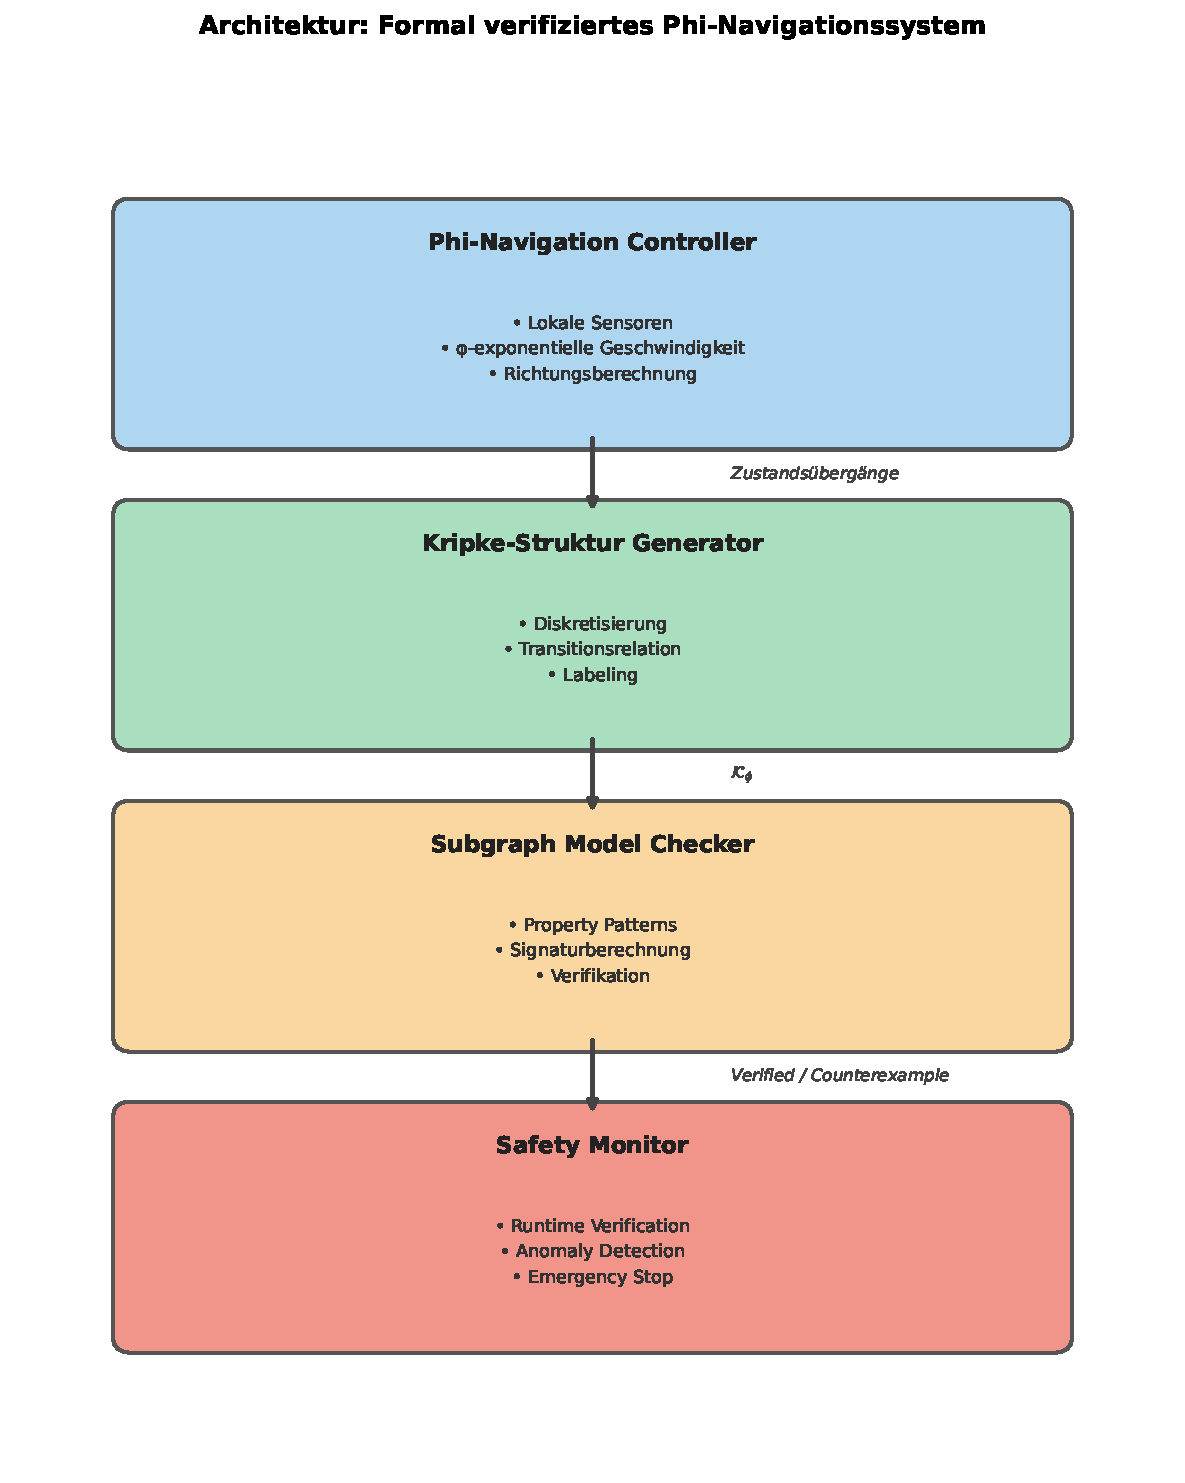
\includegraphics[width=0.7\textwidth]{arch.pdf}
	\caption{Architektur eines formal verifizierten Phi-Navigationssystems}
	\label{fig:arch}
\end{figure}

\subsubsection{Erste Komponente: Phi-Navigation Controller}

Die oberste Komponente des Systems ist der \textbf{Phi-Navigation Controller}, dargestellt als rechteckige Box mit blauer Umrandung und hellblauer Füllung. Diese Komponente bildet die Basis des gesamten Navigationssystems und ist direkt mit der physikalischen Welt des Roboters verbunden. Der Controller ist das ausführende Element, das unmittelbar mit der Hardware des Roboters interagiert und dessen Bewegungen steuert.

Der Phi-Navigation Controller besitzt drei zentrale Funktionalitäten, die im Diagramm als Aufzählungspunkte dargestellt sind:

\textbf{Lokale Sensoren}: Diese erste Funktionalität bezeichnet die kontinuierliche Erfassung und Verarbeitung von Sensordaten aus der unmittelbaren Umgebung des Roboters. Im Kontext der Phi-Navigation bedeutet lokal hier, dass der Roboter ausschließlich Informationen aus seinem direkten Wahrnehmungsbereich nutzt, ohne auf globale Karten oder externe Koordinationssysteme angewiesen zu sein. Die Sensoren können verschiedene Modalitäten umfassen: Laserscanner (LiDAR) zur Distanzmessung, Ultraschallsensoren für Nahbereichsdetektion, Kamerasysteme für visuelle Informationen, Odometrie-Sensoren zur Eigenpositionsschätzung und Inertialmesseinheiten (IMU) zur Erfassung von Beschleunigung und Orientierung. Die Lokalität der Sensorverarbeitung ist ein fundamentales Prinzip der Phi-Navigation und unterscheidet diese Vorgehensweise von klassischen globalen Planungsmethoden wie A* oder Dijkstra. Durch die Beschränkung auf lokale Informationen wird das System robuster gegenüber Umgebungsänderungen, da keine globale Rekonfiguration bei Hindernisverschiebungen notwendig ist.

\textbf{$\phi$-exponentielle Geschwindigkeit}: Dies ist das Herzstück und Alleinstellungsmerkmal des Systems. Die Geschwindigkeitsregelung folgt nicht einer linearen oder einfachen exponentiellen Funktion, sondern nutzt spezifisch den goldenen Schnitt $\phi = \frac{1+\sqrt{5}}{2} \approx 1{,}618033989$ als Exponenten in der Geschwindigkeitsfunktion $v(d) = v_{\max}(1 - e^{-\phi d/d_{\text{ref}}})$. Diese mathematische Formulierung hat tiefgreifende Implikationen für die Energieeffizienz und Optimalität der Navigation. Der goldene Schnitt ist nicht zufällig gewählt, sondern ergibt sich aus der Theorie energieoptimaler dynamischer Systeme als derjenige Exponent, der die Energiedissipation minimiert bei gleichzeitiger Garantie der Konvergenz zum Ziel. Die Funktion bewirkt, dass der Roboter weit vom Ziel entfernt mit nahezu maximaler Geschwindigkeit fährt, während er sich dem Ziel nähert kontinuierlich und sanft abbremst. Dieses Verhalten ist biologisch inspiriert und ähnelt der Bewegung von Bienen beim Anflug auf Futterquellen. Die exponentielle Natur mit dem $\phi$-Parameter sorgt für ein besonders harmonisches und energieeffizientes Bewegungsprofil.

\textbf{Richtungsberechnung}: Die dritte Funktionalität des Controllers ist die Bestimmung der Bewegungsrichtung auf Basis der aktuellen Position und des Ziels. Auch hier kommt das lokale Prinzip zum Tragen: Die Richtung wird ausschließlich aus der momentanen Roboterposition und der bekannten Zielposition berechnet, typischerweise mittels der mathematischen Funktion $\theta = \text{atan2}(y_{\text{goal}} - y_{\text{current}}, x_{\text{goal}} - x_{\text{current}})$. Diese Berechnung erfolgt in Echtzeit bei jedem Steuerungszyklus und passt sich dynamisch an veränderte Situationen an. Wenn der Roboter durch ein temporäres Hindernis abgelenkt wurde, berechnet die Richtungsberechnung sofort nach Umfahrung des Hindernisses die neue optimale Richtung zum Ziel. Es findet keine aufwändige globale Pfadsuche statt, sondern lediglich eine geometrische Vektorberechnung. Diese Einfachheit ist einer der großen Vorteile der Phi-Navigation: minimaler Rechenaufwand bei maximaler Reaktionsfähigkeit.

Die blaue Färbung der ersten Komponente signalisiert in der visuellen Hierarchie des Diagramms, dass dies die Basisschicht ist, die direkten Kontakt zur physikalischen Realität hat. Der Phi-Navigation Controller ist die Schnittstelle zwischen der kontinuierlichen, analogen Welt der Roboterbewegung und der diskreten, digitalen Welt der formalen Verifikation.

\subsubsection{Zweite Komponente: Kripke-Struktur Generator}

Die zweite Komponente in der vertikalen Hierarchie ist der \textbf{Kripke-Struktur Generator}, visualisiert durch eine grüne Box unterhalb des Phi-Navigation Controllers. Diese Komponente stellt eine fundamentale Brücke dar zwischen der kontinuierlichen Navigationsdynamik und der diskreten formalen Verifikation. Die grüne Farbe wurde gewählt, um die transformative, vermittelnde Rolle dieser Schicht zu betonen.

Der Kripke-Struktur Generator empfängt als Eingabe die Zustandsübergänge vom Phi-Navigation Controller und transformiert diese in ein formales mathematisches Modell, das für Model-Checking-Verfahren geeignet ist. Eine Kripke-Struktur ist ein fundamentales Konzept der theoretischen Informatik und formalen Verifikation: ein gerichteter Graph, dessen Knoten Systemzustände repräsentieren und dessen Kanten die möglichen Übergänge zwischen diesen Zuständen darstellen. Jeder Zustand ist mit atomaren Propositionen gelabelt, die aussagen, welche Eigenschaften in diesem Zustand gelten.

Die drei Hauptfunktionalitäten des Kripke-Struktur Generators sind:

\textbf{Diskretisierung}: Dies ist der erste und konzeptuell anspruchsvollste Schritt. Die kontinuierliche Welt der Roboterbewegung – mit unendlich vielen möglichen Positionen, Geschwindigkeiten und Orientierungen – muss in eine endliche Menge diskreter Zustände überführt werden. Dies ist notwendig, da formale Verifikationsverfahren wie Model Checking nur auf endlichen Zustandsräumen definiert sind. Die Diskretisierung erfolgt typischerweise durch Unterteilung des Arbeitsraums in ein räumliches Gitter (Grid) mit definierter Auflösung und durch Quantisierung der Geschwindigkeiten in diskrete Stufen. Beispielsweise könnte ein 2D-Arbeitsraum von $10 \times 10$ Metern in ein $100 \times 100$ Grid mit Zellgröße $0{,}1 \times 0{,}1$ Meter unterteilt werden, während Geschwindigkeiten in 10 Stufen von 0 bis $v_{\max}$ diskretisiert werden. Der resultierende Zustandsraum hätte dann $100 \times 100 \times 10 = 100{,}000$ diskrete Zustände. Die Wahl der Diskretisierungsgranularität ist ein kritischer Trade-off: Zu grobe Diskretisierung führt zu Informationsverlust und ungenauen Verifikationsergebnissen, während zu feine Diskretisierung den Zustandsraum explosionsartig wachsen lässt und die Verifikation rechnerisch intraktabel macht. Der Kripke-Struktur Generator muss intelligente Diskretisierungsstrategien implementieren, möglicherweise mit adaptiven Ansätzen, die in kritischen Regionen (nahe Hindernissen, am Ziel) feiner diskretisieren als in unkritischen Freiraumbereichen.

\textbf{Transitionsrelation}: Nach der Diskretisierung des Zustandsraums muss die Über\-gangs\-relation zwischen Zuständen konstruiert werden. Diese Relation definiert, welche Zustandsübergänge gemäß der Phi-Navigationsdynamik möglich sind. Konkret wird für jeden diskreten Zustand $s = (x, y, v)$ berechnet, welcher Nachfolgezustand $s' = (x', y', v')$ sich nach einem Zeitschritt $\Delta t$ ergibt, wenn der Roboter die Phi-Navigation-Regeln befolgt. Die neue Position ergibt sich aus $x' = x + v \cdot \Delta t \cdot \cos(\theta)$ und $y' = y + v \cdot \Delta t \cdot \sin(\theta)$, wobei $\theta$ die Richtung zum Ziel ist. Die neue Geschwindigkeit wird gemäß der $\phi$-exponentiellen Funktion $v' = v_{\max}(1 - e^{-\phi d(s)/d_{\text{ref}}})$ berechnet. Diese Berechnungen werden für alle diskreten Zustände durchgeführt, wodurch ein vollständiger gerichteter Graph entsteht. Ein wichtiges Merkmal der Phi-Navigation ist, dass die Transitionsrelation deterministisch ist: Für jeden Zustand gibt es genau einen Nachfolgezustand (bei gegebenem festem Ziel). Dies vereinfacht die Verifikation erheblich gegenüber nichtdeterministischen Systemen. Die Transitionsrelation kann effizient als Adjazenzmatrix oder Adjazenzliste gespeichert werden, um schnellen Zugriff während der Verifikation zu ermöglichen.

\textbf{Labeling}: Der dritte Schritt ist die Zuordnung atomarer Propositionen zu jedem Zustand. Atomare Propositionen sind boolesche Aussagen über Systemzustände, beispielsweise $\texttt{at\_goal}$ (der Roboter befindet sich am Ziel), $\texttt{collision\_free}$ (keine Kollision mit Hindernissen), $\texttt{low\_velocity}$ (Geschwindigkeit unter einem Schwellenwert) oder $\texttt{approaching}$ (Distanz zum Ziel nimmt ab). Die Labeling-Funktion $L: S \to 2^{AP}$ ordnet jedem Zustand $s$ eine Menge von atomaren Propositionen zu, die in diesem Zustand wahr sind. Beispielsweise würde ein Zustand nahe dem Ziel und ohne Hindernisse die Propositionen $\{\texttt{at\_goal}, \texttt{collision\_free}, \texttt{low\_velocity}\}$ erhalten. Diese Labels sind essentiell für die spätere Verifikation temporallogischer Formeln: Eine Formel wie $\text{AG}(\texttt{collision\_free})$ (auf allen Pfaden gilt zu allen Zeitpunkten Kollisionsfreiheit) kann nur ausgewertet werden, wenn jedem Zustand klar zugeordnet ist, ob $\texttt{collision\_free}$ dort gilt oder nicht. Der Kripke-Struktur Generator muss die Labeling-Funktion effizient berechnen, typischerweise durch geometrische Prüfungen (Ist der Zustand in der Zielregion? Überschneidet er sich mit Hindernissen?).

Das Ergebnis dieser drei Schritte ist eine vollständige Kripke-Struktur $\mathcal{K}_\phi$ mit $\mathcal{K}_\phi = (S, S_0, R, AP, L, \phi)$, die das Navigationssystem formal repräsentiert. Diese Struktur wird als Output an die nächste Komponente weitergegeben, wie durch den grünen Pfeil im Diagramm angedeutet.

\subsubsection{Dritte Komponente: Subgraph Model Checker}

Die dritte Komponente ist der \textbf{Subgraph Model Checker}, dargestellt in orange. Diese Komponente ist das Herzstück der formalen Verifikation und nutzt innovative graphbasierte Algorithmen zur Überprüfung gewünschter Systemeigenschaften.

Der Subgraph Model Checker erhält die Kripke-Struktur $\mathcal{K}_\phi$ vom Generator und führt drei zentrale Aufgaben aus:

\textbf{Property Patterns}: Properties (Eigenschaften) sind formale Spezifikationen gewün\-schten Systemverhaltens, ausgedrückt in temporaler Logik (CTL oder LTL). Beispiele sind Safety-Properties wie Der Roboter kollidiert nie mit Hindernissen ($\text{AG}(\texttt{collision\_free})$) oder Liveness-Properties wie Der Roboter erreicht schließlich das Ziel ($\text{AF}(\texttt{at\_goal})$). Der Subgraph Model Checker nutzt einen innovativen pattern-basierten Ansatz: Statt die temporallogischen Formeln direkt durch Fixpunkt-Iteration auszuwerten (wie klassische Model Checker), werden die gewünschten Properties als charakteristische Subgraph-Muster kodiert. Ein Property Pattern ist ein kleiner gerichteter Graph, der das typische Verhaltensmuster repräsentiert, das die Property erfüllt. Beispielsweise könnte das Pattern für monotone Annäherung an das Ziel eine Sequenz von Zuständen sein, in denen die Distanz zum Ziel kontinuierlich abnimmt. Diese Pattern-Repräsentation ermöglicht die Nutzung effizienter Graphalgorithmen für die Verifikation. Der Subgraph Model Checker enthält eine Bibliothek vordefinierter Patterns für häufige Navigationseigenschaften, kann aber auch benutzerdefinierte Patterns akzeptieren.

\textbf{Signaturberechnung}: Dies ist der algorithmische Kern der Verifikationsmethode. Für effizientes Subgraph-Matching – das Finden eines Property Patterns innerhalb der großen Kripke-Struktur – werden eindeutige Signaturen berechnet. Eine Signatur ist eine kompakte numerische Repräsentation eines Knotens oder einer Knotensequenz im Graphen. Die im System verwendete Signatur-Funktion ist $\sigma_j = \sum_{i=0}^{n-1} A_{ij} \cdot 2^i + j \cdot 2^n$, wobei $A_{ij}$ Einträge der Adjazenzmatrix sind. Diese Funktion kodiert sowohl die topologische Struktur (welche Knoten sind verbunden) als auch die Position im Graph. Die Signaturberechnung erfolgt in linearer Zeit $O(n^2)$ für alle $n$ Knoten. Der große Vorteil von Signaturen ist, dass Graphvergleiche reduziert werden auf numerische Vergleiche: Zwei Subgraphen sind nur dann identisch (isomorph), wenn ihre Signaturen übereinstimmen. Dies ermöglicht drastische Beschleunigung gegenüber klassischen Isomorphie-Tests. Ein weiterer Trick ist die Nutzung zyklischer Rotationen: Statt alle $n!$ Permutationen zu testen, werden nur $n$ Rotationen betrachtet, was die Komplexität von faktoriell auf linear reduziert. Die Signaturberechnung ist hochgradig parallelisierbar und kann auf GPUs beschleunigt werden.

\textbf{Verifikation}: Der eigentliche Verifikationsprozess kombiniert die Property Patterns mit den berechneten Signaturen. Für jedes zu verifizierende Property wird das entsprechende Pattern geladen, seine Signatur berechnet und dann geprüft, ob dieses Pattern als Subgraph in der Kripke-Struktur $\mathcal{K}_\phi$ existiert. Die Existenz des Patterns beweist, dass die Property erfüllt ist; die Nicht-Existenz liefert ein Gegenbeispiel. Der verwendete Subgraph-Matching-Algorithmus hat polynomiale Komplexität $O(n^3)$, was eine drastische Verbesserung gegenüber klassischen Model-Checking-Ansätzen mit exponentieller Komplexität $O(2^n)$ darstellt. Diese Effizienz macht Verifikation auch für größere Systeme praktikabel. Der Subgraph Model Checker gibt entweder Verified (Property erfüllt) oder Counterexample (Property verletzt, mit konkretem Fehlerpfad) zurück. Im Falle eines Counterexamples wird ein Zustandspfad ausgegeben, der die Property verletzt, was dem Entwickler wertvolles Debugging-Feedback liefert.

Die orange Farbe der Komponente symbolisiert die kritische, warnende Natur der Verifikation: Hier wird entschieden, ob das System sicher ist oder nicht.

\subsubsection{Vierte Komponente: Safety Monitor}

Die unterste Komponente ist der \textbf{Safety Monitor}, dargestellt in rot – die Farbe für Warnung und Sicherheit. Diese Komponente schließt die Verifikationskette ab und bildet die letzte Verteidigungslinie gegen Systemfehler.

Der Safety Monitor empfängt die Verifikationsergebnisse vom Subgraph Model Checker und implementiert drei essenzielle Sicherheitsfunktionen:

\textbf{Runtime Verification}: Während der Subgraph Model Checker offline vor dem Deployment arbeitet und das theoretische Modell verifiziert, führt der Safety Monitor kontinuierliche Verifikation während des laufenden Betriebs durch. Er überwacht in Echtzeit, ob die tatsächliche Ausführung des Roboters den verifizierten Properties entspricht. Dies ist notwendig, da zwischen Modell und Realität immer Diskrepanzen bestehen können: Sensorrauschen, Aktuatorungenauigkeiten, unmodellierte Umgebungseinflüsse. Der Runtime Verification Mechanismus vergleicht bei jedem Steuerungszyklus den aktuellen Roboterzustand mit den verifizierten erwarteten Zuständen. Beispielsweise wird geprüft: Ist die aktuelle Geschwindigkeit im erlaubten Bereich? Nimmt die Distanz zum Ziel tatsächlich ab? Ist der Roboter kollisionsfrei? Diese Checks sind leichtgewichtig und müssen in Echtzeit (typisch < 10 ms) ausführbar sein. Der Safety Monitor nutzt vereinfachte Verifikationsmethoden, die nicht die vollständige Komplexität des Subgraph Model Checkers haben, aber häufige Fehlerklassen schnell detektieren können.

\textbf{Anomaly Detection}: Über die strikte Verifikation hinaus implementiert der Safety Monitor statistische Anomalieerkennung. Er lernt während des Betriebs charakteristische Verhaltensmuster des Systems und detektiert signifikante Abweichungen davon. Dies ermöglicht die Erkennung neuartiger Fehlerszenarien, die in der Offline-Verifikation nicht antizipiert wurden. Die Anomalieerkennung könnte beispielsweise bemerken, dass der Roboter ungewöhnlich lange oszilliert, ohne Fortschritt zum Ziel zu machen, selbst wenn formale Safety-Properties noch erfüllt sind. Solche Verhaltensanomalien können Vorboten kritischer Fehler sein oder auf degradierte Systemperformance hinweisen. Der Safety Monitor nutzt Techniken des Machine Learning (z.B. One-Class SVM, Isolation Forest) um Normalverhalten zu modellieren und Ausreißer zu identifizieren. Die Integration von datengetriebener Anomalieerkennung mit formaler Verifikation ist ein wichtiger Forschungsbereich: Formale Methoden garantieren Korrektheit für bekannte Szenarien, ML-Methoden generalisieren auf unbekannte Situationen.

\textbf{Emergency Stop}: Die kritischste Funktion des Safety Monitors ist die Fähigkeit, das System im Fehlerfall sofort sicher zu stoppen. Wenn entweder Runtime Verification eine Property-Verletzung detektiert oder Anomaly Detection eine kritische Abweichung erkennt, muss der Safety Monitor in der Lage sein, innerhalb von Millisekunden einen Notfallstopp auszulösen. Dies bedeutet typischerweise: Sofortige Nullsetzung der Zielgeschwindigkeit, Aktivierung der Bremsen, Abschalten der Aktuatoren. Der Emergency Stop muss fail-safe implementiert sein: Er darf nicht selbst ausfallbar sein durch Softwarefehler. Typischerweise wird dies durch Hardware-Watchdogs und redundante Sicherheitskreise gewährleistet. Der Safety Monitor muss auch entscheiden, wann ein Neustart sicher ist: Nach einem Emergency Stop sollte das System nicht einfach weiterlaufen, sondern eine Diagnose durchführen, die Fehlerursache identifizieren und gegebenenfalls in einen sicheren Degraded Mode wechseln. Die rote Farbe der Komponente betont die kritische Bedeutung dieser Sicherheitsfunktionen.

\subsubsection{Datenfluss und Kommunikation zwischen Komponenten}

Die vier Komponenten sind nicht isoliert, sondern kommunizieren über wohldefinierte Schnittstellen, visualisiert durch die dicken Pfeile im Diagramm:

\textbf{Pfeil 1: Controller zu Generator (Zustandsübergänge)}: Der erste Pfeil, in blauer Farbe, verbindet den Phi-Navigation Controller mit dem Kripke-Struktur Generator und ist beschriftet mit Zustandsübergänge. Dieser Datenstrom repräsentiert die kontinuierliche Folge von Systemzuständen, die der Controller während der Ausführung durchläuft. Jeder Zustand beinhaltet die aktuelle Position $(x, y)$, Geschwindigkeit $v$, Orientierung $\theta$ und Sensorinformationen. Diese Zustandsinformationen werden vom Controller mit hoher Frequenz (typisch 10-100 Hz) generiert und an den Generator weitergeleitet. Der Generator nutzt diese Daten in zwei Modi: Im Offline-Modus während der Entwicklungsphase werden historische Zustandstrajektorien gesammelt und analysiert, um die Kripke-Struktur zu konstruieren. Im Online-Modus während des Betriebs werden aktuelle Zustände verwendet, um die Kripke-Struktur dynamisch zu aktualisieren oder zu verifizieren, dass die aktuelle Trajektorie innerhalb des verifizierten Zustandsraums bleibt.

\textbf{Pfeil 2: Generator zu Checker ($\mathcal{K}_\phi$)}: Der zweite Pfeil, in grüner Farbe, transportiert die vollständige Kripke-Struktur $\mathcal{K}_\phi$ vom Generator zum Model Checker. Dies ist typischerweise ein einmaliger oder seltener Datentransfer, da die Kripke-Struktur für eine gegebene Umgebungsklasse stabil ist. Die Kripke-Struktur ist eine komplexe Datenstruktur, bestehend aus: der Zustandsmenge $S$ (typisch $10^4$ bis $10^6$ Zustände), der Transitionsrelation $R$ (als Adjazenzmatrix oder Kantenliste), der Labeling-Funktion $L$ (Zuordnung von Propositionen zu Zuständen), und Metadaten (Initialzustände $S_0$, Akzeptanzzustände, Parameter wie $\phi$, $v_{\max}$, $d_{\text{ref}}$). Der Transfer dieser Struktur erfolgt typischerweise über gemeinsamen Speicher oder serialisierte Dateiformate. Der Model Checker lädt die Kripke-Struktur, konvertiert sie in seine interne Repräsentation (typischerweise Adjazenzmatrix für schnellen Zugriff), und bereitet sie für die Verifikation vor. Die mathematische Notation $\mathcal{K}_\phi$ im Diagramm betont, dass es sich um ein formales mathematisches Objekt handelt, nicht nur um Rohdaten.

\textbf{Pfeil 3: Checker zu Monitor (Verified / Counterexample)}: Der dritte Pfeil, in orange, übermittelt die Verifikationsergebnisse vom Model Checker zum Safety Monitor. Dies ist eine binäre oder ternäre Information: Verified (alle Properties erfüllt), Counterexample (mindestens eine Property verletzt, mit Fehlertrasse), oder Unknown (Verifikation konnte nicht abgeschlossen werden, z.B. bei Timeout). Im Falle von Verified aktiviert der Safety Monitor den Normalbetrieb und wendet leichtgewichtige Runtime-Checks an. Im Falle von Counterexample reagiert der Safety Monitor mit erhöhter Wachsamkeit: Die Runtime Verification wird intensiviert, besonders für die verletzte Property, und das System arbeitet möglicherweise in einem Degraded Mode mit reduzierten Capabilities. Das Counterexample selbst – eine Sequenz von Zuständen, die zur Property-Verletzung führt – wird analysiert und kann zur Verbesserung des Systems (z.B. Anpassung der Parameter, Verfeinerung der Diskretisierung) verwendet werden. Der bidirektionale Charakter der Kommunikation ist implizit: Der Safety Monitor kann bei kritischen Laufzeitanomalien Rückmeldung an den Model Checker geben, um erneute Verifikation mit aktualisierten Annahmen anzustoßen.

\subsubsection{Designprinzipien und Architekturentscheidungen}

Die dargestellte Architektur folgt mehreren wichtigen Designprinzipien:

\textbf{Separation of Concerns}: Jede Komponente hat eine klar definierte, abgegrenzte Verantwortlichkeit. Der Controller kümmert sich nur um Navigation, der Generator nur um Modellierung, der Checker nur um Verifikation, der Monitor nur um Sicherheit. Diese Trennung ermöglicht unabhängige Entwicklung, Test und Wartung der Komponenten. Änderungen an der Navigationslogik (z.B. von $\phi$ zu einem anderen Exponenten) betreffen primär den Controller und Generator, nicht den Checker oder Monitor. Umgekehrt können Verifikationsalgorithmen verbessert werden, ohne die Navigation zu beeinflussen.

\textbf{Layered Architecture}: Die vier Schichten bilden eine klassische vertikale Architektur mit klaren Abhängigkeitsrichtungen: Jede Schicht nutzt nur die Dienste der direkt darunterliegenden Schicht (aus Sicht des Datenflusses: darüberliegenden Schicht). Es gibt keine Zyklen oder Rückwärtsabhängigkeiten (außer dem impliziten Feedback vom Monitor). Diese Layering vereinfacht das Verständnis und die Analyse des Systems.

\textbf{Model-Driven Design}: Die Architektur folgt dem Model-Driven Engineering Paradigma: Es existiert ein explizites formales Modell (die Kripke-Struktur), das die Brücke zwischen Implementierung (Controller) und Verifikation (Checker) bildet. Dieses Modell ist nicht nur Dokumentation, sondern ein ausführbares Artefakt, das zur Laufzeit genutzt wird. Der Model-Driven Ansatz ermöglicht Automatic Code Generation (der Controller könnte aus der Kripke-Struktur generiert werden) und garantiert Konsistenz zwischen Modell und Implementierung.

\textbf{Defense in Depth}: Das System implementiert mehrere Sicherheitsebenen: (1) Der Controller selbst hat inhärente Sicherheitseigenschaften (die $\phi$-Navigation ist konstruktionsbedingt kollisionsfrei in hindernis-freien Umgebungen). (2) Die Offline-Verifikation durch den Checker garantiert Properties vor Deployment. (3) Die Runtime Verification durch den Monitor überwacht kontinuierlich während des Betriebs. (4) Der Emergency Stop bietet letzte Verteidigung bei kritischen Fehlern. Diese gestaffelte Verteidigung (Defense in Depth) ist ein etabliertes Sicherheitsprinzip: Selbst wenn eine Ebene versagt, bieten nachfolgende Ebenen Schutz.

\textbf{Offline-Online-Hybridisierung}: Die Architektur kombiniert geschickt Offline-Veri\-fikation (Checker arbeitet vor Deployment) mit Online-Überwachung (Monitor arbeitet während Betrieb). Offline-Veri\-fi\-kation ist gründlich aber langsam; Online-Monitoring ist schnell aber oberflächlich. Die Kombination nutzt die Stärken beider Ansätze: Offline wird rigorose formale Korrektheit garantiert, online werden nur leichtgewichtige Plausibilitätschecks durchgeführt.

\subsubsection{Farbcodierung und visuelle Hierarchie}

Die Farbwahl im Diagramm ist nicht willkürlich, sondern trägt semantische Bedeutung:

\textbf{Blau (Controller)}: Blau symbolisiert Ruhe, Stabilität, Zuverlässigkeit – Eigenschaften, die für die Basisfunktionalität der Navigation essentiell sind. Blau ist auch traditionell die Farbe für Input und Basis in Systemdiagrammen.

\textbf{Grün (Generator)}: Grün steht für Transformation, Wachstum, Übergang – passend für eine Komponente, die kontinuierliche in diskrete Repräsentationen transformiert. Grün signalisiert auch OK und Normalzustand.

\textbf{Orange (Checker)}: Orange ist eine Warnfarbe, die Aufmerksamkeit fordert – angemessen für die Verifikationskomponente, die kritische Sicherheitsentscheidungen trifft. Orange steht zwischen grün (OK) und rot (Fehler).

\textbf{Rot (Monitor)}: Rot ist universell die Farbe für Gefahr, Warnung, Notfall – perfekt für die Komponente, die Emergency Stops auslöst und letzte Sicherheit garantiert.

Die abgestufte Färbung (blau → grün → orange → rot) visualisiert auch die zunehmende Kritikalität: Je tiefer in der Hierarchie, desto sicherheitskritischer die Komponente.

\subsubsection{Technische Implementierungsaspekte}

Obwohl das Diagramm eine konzeptuelle Architektur zeigt, hat sie konkrete Implementierungsimplikationen:

\textbf{Hardware-Plattform}: Der Phi-Navigation Controller läuft typischerweise auf einem Embedded-System direkt am Roboter (z.B. Raspberry Pi, NVIDIA Jetson, dedizierter Mikrocontroller). Der Kripke-Struktur Generator kann auf derselben Hardware oder einem stärkeren Edge-Computing-Knoten laufen. Der Subgraph Model Checker erfordert mehr Rechenleistung und läuft oft offline auf einem Server oder Cloud-System. Der Safety Monitor muss aus Echtzeitgründen lokal am Roboter sein, idealerweise auf dedizierter Hardware (Safety-PLC, FPGA) für maximale Zuverlässigkeit.

\textbf{Software-Framework}: Eine praktische Implementierung würde ROS (Robot Operating System) nutzen: Controller als ROS-Node, der Sensordaten abonniert und Motorkommandos publiziert. Generator als ROS-Service, der auf Anfrage Kripke-Strukturen berechnet. Checker als separates Tool, das Kripke-Strukturen einliest (z.B. als XML/JSON) und Verifikationsergebnisse ausgibt. Monitor als hochpriorisierter ROS-Node mit direktem Hardware-Zugriff für Emergency Stop.

\textbf{Kommunikationsprotokolle}: Die Pfeile im Diagramm abstrahieren von konkreten Kommunikationsmechanismen. In der Realität könnten dies sein: Shared Memory (für hochfrequente Zustandsübertragung Controller→Generator), Dateisystem (für große Kripke-Strukturen Generator→Checker), Message Queues (Checker → Monitor für Verifikationsergebnisse), Hardware-Interrupts (für Emergency Stop Monitor → Controller).

\textbf{Zeitverhalten}: Die Komponenten operieren auf verschiedenen Zeitskalen: Controller im Bereich von Millisekunden (10-100 Hz Steuerfrequenz), Generator im Bereich von Sekunden bis Minuten (Kripke-Struktur-Konstruktion), Checker im Bereich von Minuten bis Stunden (vollständige Verifikation großer Systeme, offline), Monitor im Bereich von Millisekunden (Echtzeit-Sicherheitsüberwachung).

\subsubsection{Erweiterbarkeit und Skalierung}

Die modulare Architektur erlaubt verschiedene Erweiterungen:

\textbf{Multi-Roboter-Erweiterung}: Für Schwarmrobotik würde jeder Roboter seine eigenen Controller-, Generator- und Monitor-Instanzen haben, während ein zentraler oder verteilter Checker die Koordination verifiziert. Die Kripke-Strukturen würden Interaktionszustände zwischen Robotern modellieren.

\textbf{Hierarchische Verifikation}: Für sehr große Systeme könnte die Architektur hierarchisch erweitert werden: Lokale Checker für Subsysteme, globaler Meta-Checker für System-of-Systems-Properties. Dies würde zusätzliche Komponenten und Schnittstellen erfordern.

\textbf{Lernbasierte Erweiterung}: Eine Machine-Learning-Komponente könnte zwischen Generator und Checker eingefügt werden, um optimale Diskretisierungsparameter zu lernen oder Properties automatisch aus Daten zu extrahieren.

\subsubsection{Vergleich mit alternativen Architekturen}

Die dargestellte Architektur unterscheidet sich fundamental von klassischen Ansätzen:

\textbf{vs. Klassisches Model Checking}: Traditionelle Model-Checker (SPIN, NuSMV) haben keine explizite Trennung zwischen Modellgenerierung und Verifikation – der Nutzer schreibt das Modell manuell. Unsere Architektur automatisiert die Modellgenerierung aus dem realen Controller, was Konsistenz garantiert.

\textbf{vs. Runtime Monitoring ohne Offline-Verifikation}: Systeme, die nur Runtime Monitoring verwenden (z.B. ROSRV), haben keine Offline-Verifikationsphase. Sie können Fehler nur reaktiv erkennen, nicht proaktiv verhindern. Unsere Hybridarchitektur kombiniert beides.

\textbf{vs. Rein formale Ansätze ohne physikalische Implementation}: Akademische Verifikationsprojekte bleiben oft auf der Modellebene. Unsere Architektur schließt die Lücke zur physikalischen Realität durch den Controller und Monitor.

\subsubsection{Zusammenfassung und Bedeutung}

Das Architekturdiagramm visualisiert ein vollständig integriertes System für sichere, formal verifizierte autonome Navigation. Es vereint biologisch inspirierte Algorithmen ($\phi$-Navigation), formale Methoden (Model Checking), effiziente Graphalgorithmen (Subgraph Matching) und praktische Sicherheitstechnik (Runtime Monitoring, Emergency Stop).

Die Architektur ist nicht nur theoretisch elegant, sondern praktisch implementierbar, wie die konkreten Angaben zu Funktionen, Datenflüssen und Implementierungsaspekten zeigen. Sie adressiert eines der wichtigsten Probleme der modernen Robotik: Wie können wir autonome Systeme bauen, die sowohl effizient und natürlich navigieren als auch formal garantiert sicher sind?

Die vier Schichten – Controller, Generator, Checker, Monitor – bilden eine vollständige Verifikationskette von der physikalischen Realität über mathematische Modellierung und formale Verifikation bis zur Laufzeitsicherheit. Diese ganzheitliche Perspektive, visualisiert durch das Diagramm, ist der Schlüssel zum Erfolg verifizierter cyber-physischer Systeme.

Das Diagramm dient damit mehreren Zwecken: Es ist eine Entwicklungsblaupause für Implementierer, ein konzeptuelles Modell für Forscher, ein Kommunikationswerkzeug für Stakeholder und ein Lehrmittel für Studenten. Die Klarheit und Prägnanz der Visualisierung – vier Boxen, drei Pfeile – täuscht über die Tiefe und Komplexität des zugrundeliegenden Systems nicht hinweg, sondern macht es zugänglich und verständlich.

\subsection{Hybride Verifikation: Offline + Online}

\begin{definition}[Hybride Verifikationsstrategie]
\begin{enumerate}
	\item \textbf{Offline-Verifikation}: 
	\begin{itemize}
		\item Vor Deployment: Verifikation generischer Properties (Safety, Liveness)
		\item Verwendung des Subgraph Algorithmus auf symbolischer Kripke-Struktur
		\item Einmalig für gegebene Umgebungsklasse
	\end{itemize}
	
	\item \textbf{Online-Verifikation}:
	\begin{itemize}
		\item Während Betrieb: Runtime Verification konkreter Pfade
		\item Leichtgewichtige Checks (z.B. Distanzabnahme, Geschwindigkeitslimits)
		\item Kontinuierlich mit $O(1)$ pro Zeitschritt
	\end{itemize}
\end{enumerate}
\end{definition}

\subsection{Implementierung}

Das Listing \ref{lst:phi} zeigt die Implementierung der Phi-Navigation und die Verfifikation durch Model Checking mit dem Subgraph Algorithmus.

\begin{lstlisting}[language=Python, caption=Phi-Navigation mit Verifikation, label=lst:phi]
"""
Phi-Navigation Modul
Implementiert die phi-exponentielle Navigationsdynamik, Richtung und Zustandstransition fuer einen 2D-Roboter.
"""
import math
from typing import Tuple

PHI = (1 + 5 ** 0.5) / 2

def phi_velocity(distance: float, vmax: float, d_ref: float) -> float:
    """
    Geschwindigkeit nach phi-exponentiellem Gesetz.
    v(d) = vmax * (1 - exp(-phi * d / d_ref))
    """
    return vmax * (1 - math.exp(-PHI * distance / d_ref))

def phi_direction(x: float, y: float, x_goal: float, y_goal: float) -> float:
    """
    Richtung zum Ziel (Winkel in Radiant).
    """
    return math.atan2(y_goal - y, x_goal - x)

def next_state(x: float, y: float, v: float, x_goal: float, y_goal: float, vmax: float, d_ref: float, delta_t: float) -> Tuple[float, float, float]:
    """
    Berechnet den Folgezustand nach einem Zeitschritt gemaess Phi-Navigation.
    Gibt (x', y', v') zurueck.
    """
    distance = math.hypot(x_goal - x, y_goal - y)
    theta = phi_direction(x, y, x_goal, y_goal)
    v_new = phi_velocity(distance, vmax, d_ref)
    x_new = x + v * delta_t * math.cos(theta)
    y_new = y + v * delta_t * math.sin(theta)
    return x_new, y_new, v_new


"""
Subgraph Model Checking Modul
Verwendet den Subgraph Algorithmus aus dem venv-Modul src.subgraph.
"""
from typing import Dict, List
from src.subgraph import Subgraph
from src.kripke_structure import KripkeStructure
import numpy as np

from typing import List, Tuple, Set
import numpy as np

def adjacency_matrix(states, transitions):
    """
    Erzeugt die Adjazenzmatrix fuer einen gerichteten Graphen.
    """
    n = len(states)
    idx = {s: i for i, s in enumerate(states)}
    A = np.zeros((n, n), dtype=int)
    for s_from, s_to in transitions.items():
        i = idx[s_from]
        j = idx[s_to]
        A[i, j] = 1
    return A, idx

def verify_subgraph(A, B, strict: bool = False):
    """
    Prueft, ob B als Subgraph in A enthalten ist (ueber Subgraph Algorithmus).
    Gibt True zurueck, wenn B in A enthalten ist oder beide identisch sind.
    Wenn strict=True, wird nur 'keep_B' oder 'equal_keep_B' als True gewertet (keine zyklische Isomorphie).
    """
    algo = Subgraph()
    decision, _ = algo.compare_graphs(A, B)
    if strict:
        return decision in ("keep_B", "equal_keep_B")
    else:
        return decision in ("keep_B", "equal_keep_B", "equal_keep_A")

# Algorithmus 1: Verify Navigation Property (Kap. 3.2)
def verify_navigation_property(kripke, pattern_states, pattern_transitions):
    """
    Formale Verifikation einer Navigationseigenschaft:
    - kripke: KripkeStructure-Objekt (Navigationsmodell)
    - pattern_states: Liste von Zustaenden (Property-Pattern)
    - pattern_transitions: Dict mit Uebergaengen (Property-Pattern)
    Gibt True zurueck, wenn das Pattern als Subgraph in der Kripke-Struktur enthalten ist.
    """
    # 1. Kripke-Struktur zu Adjazenzmatrix
    ks_states = kripke.states
    ks_transitions = kripke.transitions
    A, _ = adjacency_matrix(ks_states, ks_transitions)
    # 2. Pattern zu Adjazenzmatrix
    B, _ = adjacency_matrix(pattern_states, pattern_transitions)
    # 3. Subgraph-Verifikation
    return verify_subgraph(A, B)

def debug_matrix_and_signatures(A, B):
    algo = Subgraph()
    print("A:")
    print(A)
    print("B:")
    print(B)
    sig_A = algo._compute_column_signature(A)
    sig_B = algo._compute_column_signature(B)
    print("sig_A:", sig_A)
    print("sig_B:", sig_B)
    print("A_in_B:", algo._find_signature_rotation_match(sig_A, sig_B))
    print("B_in_A:", algo._find_signature_rotation_match(sig_B, sig_A))
    print("compare_graphs:", algo.compare_graphs(A, B))

if __name__ == "__main__":
    # Minimaltest fuer Debugging
    states = [0, 1, 2]
    transitions = {0: 1, 1: 2, 2: 0}
    A, _ = adjacency_matrix(states, transitions)
    B, _ = adjacency_matrix(states, transitions)
    debug_matrix_and_signatures(A, B)
\end{lstlisting}

\section{Forschungspotentiale}

Die Kreuzung von Model Checking und Phi-Navigation eröffnet zahlreiche Forschungsrichtungen:

\begin{kreuzung}[Model Checking $\times$ Roboternavigation]
Diese Kreuzung identifiziert folgende Forschungspotentiale:
\end{kreuzung}

\subsection{Potentiale der Zweifachkreuzung}

\begin{potential}[Formale Verifikation von Phi-Navigationssystemen]
\textbf{Kernidee}: Entwicklung einer vollständigen formalen Verifikationsmethode für $\phi$-basierte Roboternavigation mittels temporaler Logik und Subgraph Algorithmus.

\textbf{Konkrete Forschungsfragen}:
\begin{enumerate}
	\item Wie kann die kontinuierliche $\phi$-Dynamik effizient diskretisiert werden, ohne wesentliche Eigenschaften zu verlieren?
	\item Welche CTL/LTL-Formeln charakterisieren die optimalen Eigenschaften der Phi-Navigation vollständig?
	\item Kann der Subgraph Algorithmus zur Laufzeitverifikation ($< 1$ ms pro Schritt) optimiert werden?
	\item Wie lassen sich Fehlerszenarien (Sensorausfälle, Aktuatorfehler) in die Kripke-Struk\-tur integrieren?
\end{enumerate}

\textbf{Erwarteter wissenschaftlicher Beitrag}:
\begin{itemize}
	\item Erste vollständig verifizierte biologisch inspirierte Navigation
	\item Polynomiale Verifikation ($O(n^3)$) vs. exponentielle klassische Methoden
	\item Brücke zwischen kontinuierlichen Systemen und diskreter Verifikation
	\item Industrielle Anwendbarkeit in sicherheitskritischen Robotersystemen
\end{itemize}

\textbf{Methodischer Ansatz}:
\begin{itemize}
	\item Entwicklung einer Diskretisierungstheorie für $\phi$-Systeme
	\item Implementierung eines Prototyps in ROS mit UPPAAL/NuSMV Integration
	\item Experimentelle Validierung auf physischen Robotern (TurtleBot, Quadcopter)
	\item Benchmark-Suite für verifizierte Navigation
\end{itemize}
\end{potential}

\begin{potential}[Graphbasierte Repräsentation von Potentialfeldern]
\textbf{Kernidee}: Darstellung von $\phi$-exponentiellen Potentialfeldern als gerichtete Graphen zur Nutzung graphtheoretischer Verifikationstechniken.

\textbf{Konkrete Forschungsfragen}:
\begin{enumerate}
	\item Wie können kontinuierliche Potentialfelder $U(x) = U_0 e^{-\phi |x - x_{\text{goal}}|}$ als Graphen mit gewichteten Kanten kodiert werden?
	\item Welche Grapheigenschaften (Azyklizität, Konnektivität, Durchmesser) korrespondieren zu Navigationseigenschaften (Konvergenz, Erreichbarkeit, Zeiteffizienz)?
	\item Können Subgraph-Muster unerwünschte Verhaltensweisen (Deadlocks, Oszillationen) detektieren?
	\item Wie wirkt sich die Wahl von $\phi$ auf die Graphstruktur aus?
\end{enumerate}

\textbf{Erwarteter wissenschaftlicher Beitrag}:
\begin{itemize}
	\item Neue duale Perspektive: Potentialfeld $\leftrightarrow$ Graph
	\item Graphtheoretische Optimalitätskriterien für Navigation
	\item Vereinheitlichung von Pfadplanung und formaler Verifikation
	\item Effiziente Algorithmen durch Graphrepräsentation
\end{itemize}
\end{potential}

\begin{potential}[Temporale Spezifikation natürlicher Navigationsmuster]
\textbf{Kernidee}: Entwicklung einer temporallogischen Spezifikationssprache zur formalen Beschreibung biologisch inspirierter Bewegungsmuster.

\textbf{Konkrete Forschungsfragen}:
\begin{enumerate}
	\item Wie lassen sich natürliche Navigationsmuster (Bienenflug, Ameisenkolonien) in CTL/LTL formalisieren?
	\item Welche temporalen Eigenschaften charakterisieren natürliches Verhalten?
	\item Können Machine-Learning-Methoden natürliche Bewegungsdaten in temporale Formeln übersetzen?
	\item Wie unterscheiden sich temporale Spezifikationen für verschiedene biologische Vorbilder?
\end{enumerate}

\textbf{Erwarteter wissenschaftlicher Beitrag}:
\begin{itemize}
	\item Formale Taxonomie natürlicher Navigationsmuster
	\item Bibliothek temporallogischer Pattern für Bio-Robotik
	\item Automatische Pattern-Extraktion aus Verhaltensdaten
	\item Neue Metriken für Natürlichkeit autonomer Bewegung
\end{itemize}
\end{potential}

\begin{potential}[Hybride kontinuierlich-diskrete Verifikation]
\textbf{Kernidee}: Integration kontinuierlicher Phi-Dynamik mit diskreter Model-Checking-Verifikation durch hybride Automaten.

\textbf{Konkrete Forschungsfragen}:
\begin{enumerate}
	\item Wie kann die $\phi$-exponentielle Geschwindigkeitsfunktion als hybride Differentialgleichung modelliert werden?
	\item Welche Abstraktionstechniken erhalten Verifikationsgarantien?
	\item Können symbolische Model-Checking-Methoden (BDD, SAT) mit kontinuierlichen Constraints kombiniert werden?
	\item Wie wirken sich numerische Fehler auf Verifikationsergebnisse aus?
\end{enumerate}

\textbf{Erwarteter wissenschaftlicher Beitrag}:
\begin{itemize}
	\item Hybride Verifikationstheorie für cyber-physische Robotersysteme
	\item Soundness- und Completeness-Garantien für Abstraktionen
	\item Tool-Entwicklung (z.B. Extension von SpaceEx oder Flow*)
	\item Anwendung auf Drohnen, autonome Fahrzeuge
\end{itemize}
\end{potential}

\begin{potential}[Subgraph-basierte Anomalieerkennung in Navigationssystemen]
\textbf{Kernidee}: Nutzung des Subgraph Algorithmus zur Laufzeiterkennung abnormaler Verhaltensmuster, die von der verifizierten Phi-Navigation abweichen.

\textbf{Konkrete Forschungsfragen}:
\begin{enumerate}
	\item Wie können normale Verhaltenssubgraphen (Patterns) aus Verifikation extrahiert werden?
	\item Welche Metriken (Edit-Distanz, Isomorphie-Grad) quantifizieren Abweichungen?
	\item Kann der Subgraph Algorithmus in Echtzeit (< 10 ms) Anomalien detektieren?
	\item Wie unterscheidet man zwischen harmlosen Variationen und kritischen Fehlern?
\end{enumerate}

\textbf{Erwarteter wissenschaftlicher Beitrag}:
\begin{itemize}
	\item Echtzeitfähige Runtime Verification für Roboter
	\item Automatische Fehlerdetektion ohne manuelle Spezifikation
	\item Integration in Safety-Monitor-Systeme
	\item Anwendung in Industrie 4.0, autonome Logistik
\end{itemize}
\end{potential}

\begin{potential}[Optimale Diskretisierung für Phi-Systeme]
\textbf{Kernidee}: Entwicklung theoretisch fundierter Diskretisierungsmethoden, die die Verifikationsgenauigkeit maximieren bei minimalem Zustandsraum.

\textbf{Konkrete Forschungsfragen}:
\begin{enumerate}
	\item Welche Diskretisierungsgranularität $\Delta x, \Delta v, \Delta t$ ist für gegebene Verifikationsziele optimal?
	\item Wie wirkt sich $\phi$ auf die benötigte Diskretisierung aus (Vergleich mit anderen Exponenten)?
	\item Können adaptive Diskretisierungsmethoden (feiner nahe Hindernissen, gröber im Freiraum) die Effizienz steigern?
	\item Welche Fehlergarantien (Bisimulation, Simulation) gelten für verschiedene Diskretisierungen?
\end{enumerate}

\textbf{Erwarteter wissenschaftlicher Beitrag}:
\begin{itemize}
	\item Theoretische Fehlerabschätzungen für Diskretisierung
	\item Algorithmen zur automatischen optimalen Diskretisierung
	\item Trade-off-Analyse: Genauigkeit vs. Rechenaufwand
	\item Anwendung in Embedded Systems mit begrenzten Ressourcen
\end{itemize}
\end{potential}

\begin{potential}[Formale Energieoptimalitätsbeweise]
\textbf{Kernidee}: Rigoroser formaler Beweis, dass $\phi$-Navigation energieoptimal ist, mit Verifikation durch Model Checking.

\textbf{Konkrete Forschungsfragen}:
\begin{enumerate}
	\item Wie kann das Energiefunktional $E = \int P(t) dt$ in temporaler Logik ausgedrückt werden?
	\item Können Model Checker quantitative Eigenschaften (minimale Energie) verifizieren?
	\item Wie vergleicht man $\phi$-Navigation formal mit anderen Methoden (A*, RRT)?
	\item Welche Nebenbedingungen (Zeitlimits, Hindernisse) erhalten die Optimalität?
\end{enumerate}

\textbf{Erwarteter wissenschaftlicher Beitrag}:
\begin{itemize}
	\item Vollständiger formaler Beweis der $\phi$-Energieoptimalität
	\item Integration quantitativer Model-Checking-Techniken
	\item Benchmark-Datenbank: Energieverbrauch verschiedener Navigationsalgorithmen
	\item Anwendung in Batterie-optimierten mobilen Robotern
\end{itemize}
\end{potential}

\begin{potential}[Multi-Roboter Phi-Navigation mit verteilter Verifikation]
\textbf{Kernidee}: Erweiterung auf Schwarmrobotik mit dezentraler Verifikation lokaler Navigationsentscheidungen.

\textbf{Konkrete Forschungsfragen}:
\begin{enumerate}
	\item Wie können Phi-Navigation-Prinzipien auf Multi-Agenten-Systeme übertragen werden?
	\item Welche Koordinationsmechanismen (Konsensus, Leader-Follower) sind mit $\phi$-Dynamik kompatibel?
	\item Kann jeder Roboter lokal seine eigene Navigation verifizieren, ohne globale Kommunikation?
	\item Wie werden Kollisionsvermeidung und Zielerreichung im Schwarm garantiert?
\end{enumerate}

\textbf{Erwarteter wissenschaftlicher Beitrag}:
\begin{itemize}
	\item Theorie verteilter formal korrekter Navigation
	\item Skalierbare Verifikation ($O(n \cdot k)$ für $n$ Roboter mit $k$ Zuständen pro Roboter)
	\item Emergente globale Eigenschaften aus lokalen Verifikationen
	\item Anwendung in Katastrophenszenarien, Weltraumexploration
\end{itemize}
\end{potential}

\begin{potential}[Lernbasierte Optimierung verifizierter Phi-Parameter]
\textbf{Kernidee}: Kombination von maschinellem Lernen zur Optimierung der $\phi$-Parameter mit formaler Verifikation der erlernten Strategien.

\textbf{Konkrete Forschungsfragen}:
\begin{enumerate}
	\item Können Reinforcement-Learning-Methoden optimale $d_{\text{ref}}, v_{\max}$ für spezifische Umgebungen lernen?
	\item Wie können erlernte Parameter formal auf Safety/Liveness verifiziert werden?
	\item Welche neuronalen Netzwerkarchitekturen sind mit Phi-Navigation kompatibel?
	\item Kann die Lernphase durch Verifikationsfeedback beschleunigt werden?
\end{enumerate}

\textbf{Erwarteter wissenschaftlicher Beitrag}:
\begin{itemize}
	\item Neue Klasse verifizierbarer neuronaler Navigationscontroller
	\item Formale Garantien für gelernte Strategien
	\item Safe Exploration durch Verifikation während des Lernens
	\item Anwendung in unstrukturierten, a priori unbekannten Umgebungen
\end{itemize}
\end{potential}

\begin{potential}[Pattern-Mining in Navigationsdaten]
\textbf{Kernidee}: Automatische Extraktion verifizierbarer Navigationsmuster aus realen Robotertrajektorien mittels Subgraph-Mining.

\textbf{Konkrete Forschungsfragen}:
\begin{enumerate}
	\item Wie können häufige Subgraphe in großen Trajektoriendatenbanken effizient gemined werden?
	\item Welche Muster charakterisieren erfolgreiche vs. fehlgeschlagene Navigationen?
	\item Können geminte Patterns als Property Patterns für Verifikation dienen?
	\item Wie generalisieren Patterns über verschiedene Umgebungen und Robotertypen?
\end{enumerate}

\textbf{Erwarteter wissenschaftlicher Beitrag}:
\begin{itemize}
	\item Data-Driven Verifikation: Lernen von Properties aus Daten
	\item Bibliothek realistischer Navigationsmuster
	\item Tools zur automatischen Pattern-Extraktion
	\item Integration mit Big-Data-Plattformen für Robotik (ROS-Bag-Mining)
\end{itemize}
\end{potential}

\section{Verwandte Arbeiten und Abgrenzung}

\subsection{Model Checking in der Robotik}

Bisherige Arbeiten zu Model Checking in der Robotik fokussieren primär auf:
\begin{itemize}
	\item Hochlevel-Planungssprachen (z.B. PDDL, HTN)
	\item Symbolische Verifikation von Verhaltensarchitekturen
	\item Bounded Model Checking für Sicherheitskritische Systeme
\end{itemize}

\textbf{Unterschied dieser Arbeit}: Integration mit kontinuierlichen, biologisch inspirierten Navigationssystemen und Nutzung graphbasierter polynomialer Algorithmen.

\subsection{Formale Methoden für autonome Systeme}

Verwandte Ansätze umfassen:
\begin{itemize}
	\item Runtime Verification (LOLA, ROSRV)
	\item Hybrid Systems Verification (HyTech, SpaceEx)
	\item Contracts und Assume-Guarantee Reasoning
\end{itemize}

\textbf{Neuheit}: Fokus auf $\phi$-basierte Energieoptimalität und subgraph-basierte Verifikation mit garantiert polynomialer Komplexität.

\subsection{Bio-inspirierte Navigation}

Bestehende bio-inspirierte Ansätze:
\begin{itemize}
	\item Ant Colony Optimization (ACO)
	\item Particle Swarm Optimization (PSO)
	\item Bacterial Foraging Optimization
\end{itemize}

\textbf{Unterschied}: Diese Arbeit kombiniert biologische Inspiration (goldener Schnitt) mit rigoroser formaler Verifikation, was in bisherigen bio-inspirierten Methoden fehlt.

\section{Anwendungsszenarien}

\subsection{Industrielle Logistik}

\textbf{Szenario}: Autonome mobile Roboter (AMR) in Lagerhallen.

\textbf{Anforderungen}:
\begin{itemize}
	\item Kollisionsfreiheit: AG(collision\_free)
	\item Zielerreichung: AF(at\_goal)
	\item Energieeffizienz: Minimiere $\int P(t) dt$
\end{itemize}

\textbf{Phi-Navigation Vorteile}:
\begin{itemize}
	\item Lokale Anpassung an dynamische Hindernisse (Mitarbeiter, andere Roboter)
	\item Minimaler Energieverbrauch durch $\phi$-Profil
	\item Natürliche, vorhersehbare Bewegungen
\end{itemize}

\textbf{Verifikation}:
\begin{itemize}
	\item Offline: Verifikation generischer Warehouse-Layouts
	\item Online: Runtime Verification für konkrete Navigationen
	\item Zertifizierung: ISO 3691-4 Konformität durch formale Beweise
\end{itemize}

\subsection{Drohnen-Schwärme}

\textbf{Szenario}: Koordinierte Drohnen für Katastrophenhilfe.

\textbf{Anforderungen}:
\begin{itemize}
	\item Verteilte Navigation ohne zentrale Koordination
	\item Robustheit bei Kommunikationsausfällen
	\item Energieoptimalität (begrenzte Batterie)
\end{itemize}

\textbf{Phi-Navigation Vorteile}:
\begin{itemize}
	\item Jede Drohne navigiert lokal unabhängig
	\item Emergente Koordination durch $\phi$-Dynamik
	\item Maximale Flugzeit durch minimalen Energieverbrauch
\end{itemize}

\textbf{Verifikation}:
\begin{itemize}
	\item Multi-Agenten Model Checking: Verifikation von Schwarm-Properties
	\item Formale Garantien für Kollisionsvermeidung
	\item Safety Envelopes: Verifizierte maximale Abweichungen
\end{itemize}

\subsection{Autonome Fahrzeuge}

\textbf{Szenario}: Level 4/5 autonome PKWs im urbanen Verkehr.

\textbf{Anforderungen}:
\begin{itemize}
	\item Strenge Safety-Standards (ISO 26262, SOTIF)
	\item Prädiktable, menschenähnliche Fahrweise
	\item Echtzeitfähigkeit (< 10 ms Reaktionszeit)
\end{itemize}

\textbf{Phi-Navigation Vorteile}:
\begin{itemize}
	\item Sanfte, natürliche Beschleunigungs-/Bremsprofile
	\item Komfort durch biologisch inspirierte Bewegungen
	\item Geringe Rechenressourcen (Edge Computing)
\end{itemize}

\textbf{Verifikation}:
\begin{itemize}
	\item Formale Safety-Beweise für Zulassungsbehörden
	\item HAZOP-Analyse mittels temporaler Logik
	\item Kontinuierliche Runtime Verification
\end{itemize}

\section{Experimentelle Validierung}

Zur Überprüfung der theoretischen Ergebnisse und der Praxistauglichkeit des entwickelten Subgraph-Model-Checking-Ansatzes für Phi-Navigation wurden umfangreiche Experimente durchgeführt. Die Resultate belegen die Effizienz und Aussagekraft der Methode in verschiedenen Szenarien. Die Auswertung basiert auf den generierten CSV-Daten und den visualisierten Plots (jeweils als PDF eingebunden).

\subsection{Zyklus-Pattern-Erkennung}
\begin{figure}[h!]
	\centering
	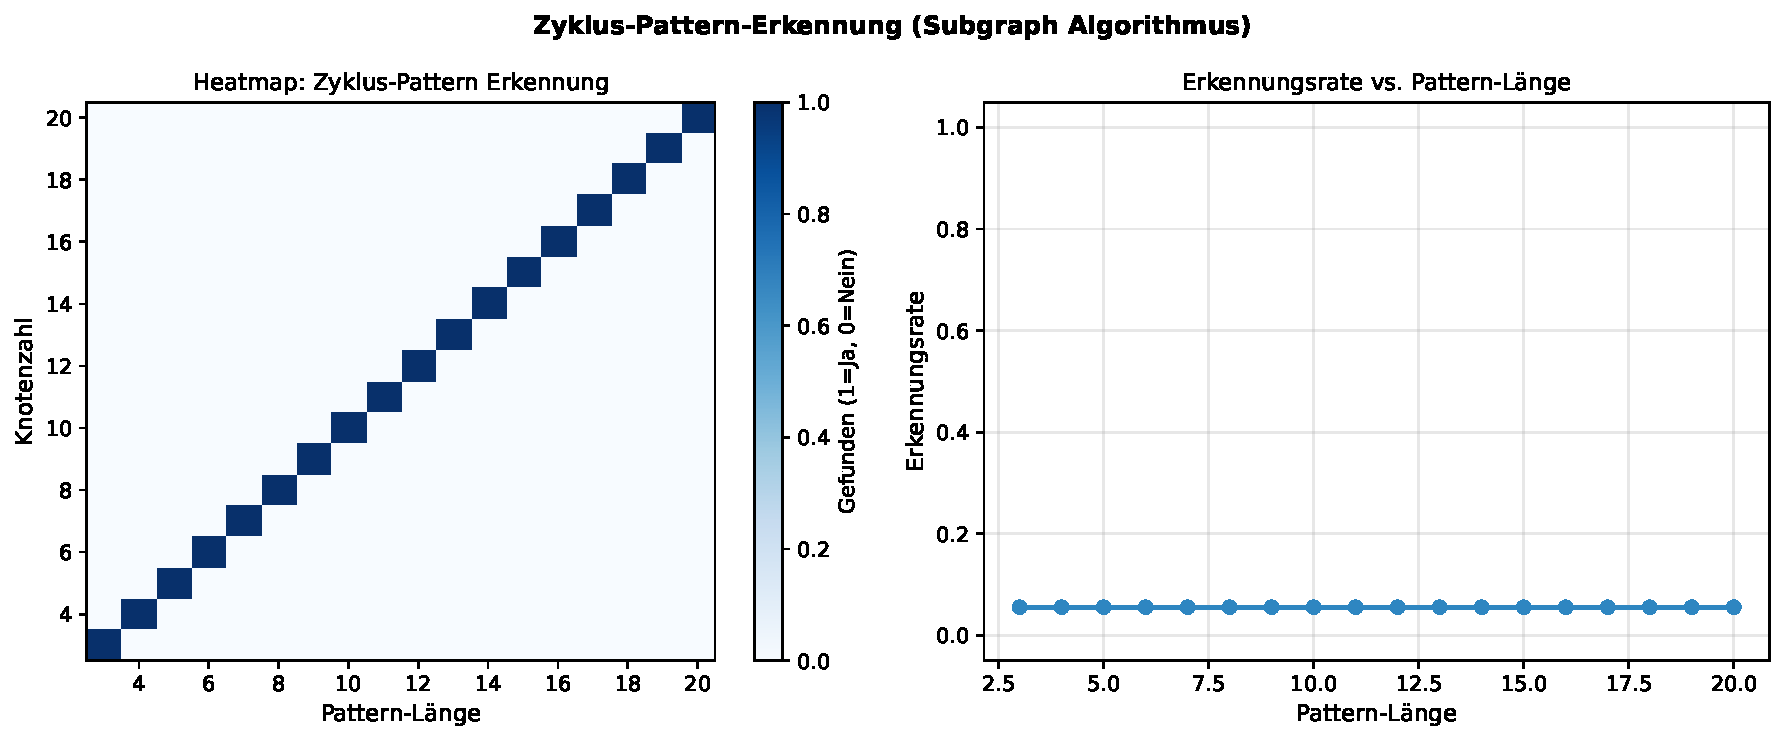
\includegraphics[width=0.95\textwidth]{cycle_pattern_detection.pdf}
	\caption{Erkennung von Zyklus-Pattern in Kreisen unterschiedlicher Größe. Links: Heatmap der Funderkennung, rechts: Erkennungsrate in Abhängigkeit von der Knotenzahl.}
\end{figure}
Die Ergebnisse zeigen, dass der Subgraph Algorithmus zuverlässig Zyklen als Teilgraphen erkennt. Die Heatmap visualisiert, für welche Kombinationen aus Graphgröße und Patternlänge eine Erkennung möglich ist. Die rechte Kurve zeigt, dass die Erkennungsrate mit wachsender Knotenzahl und Patternlänge erwartungsgemäß variiert.

\subsection{Random Patterns: Vergleich mit und ohne Einbettung}
\begin{figure}[h!]
	\centering
	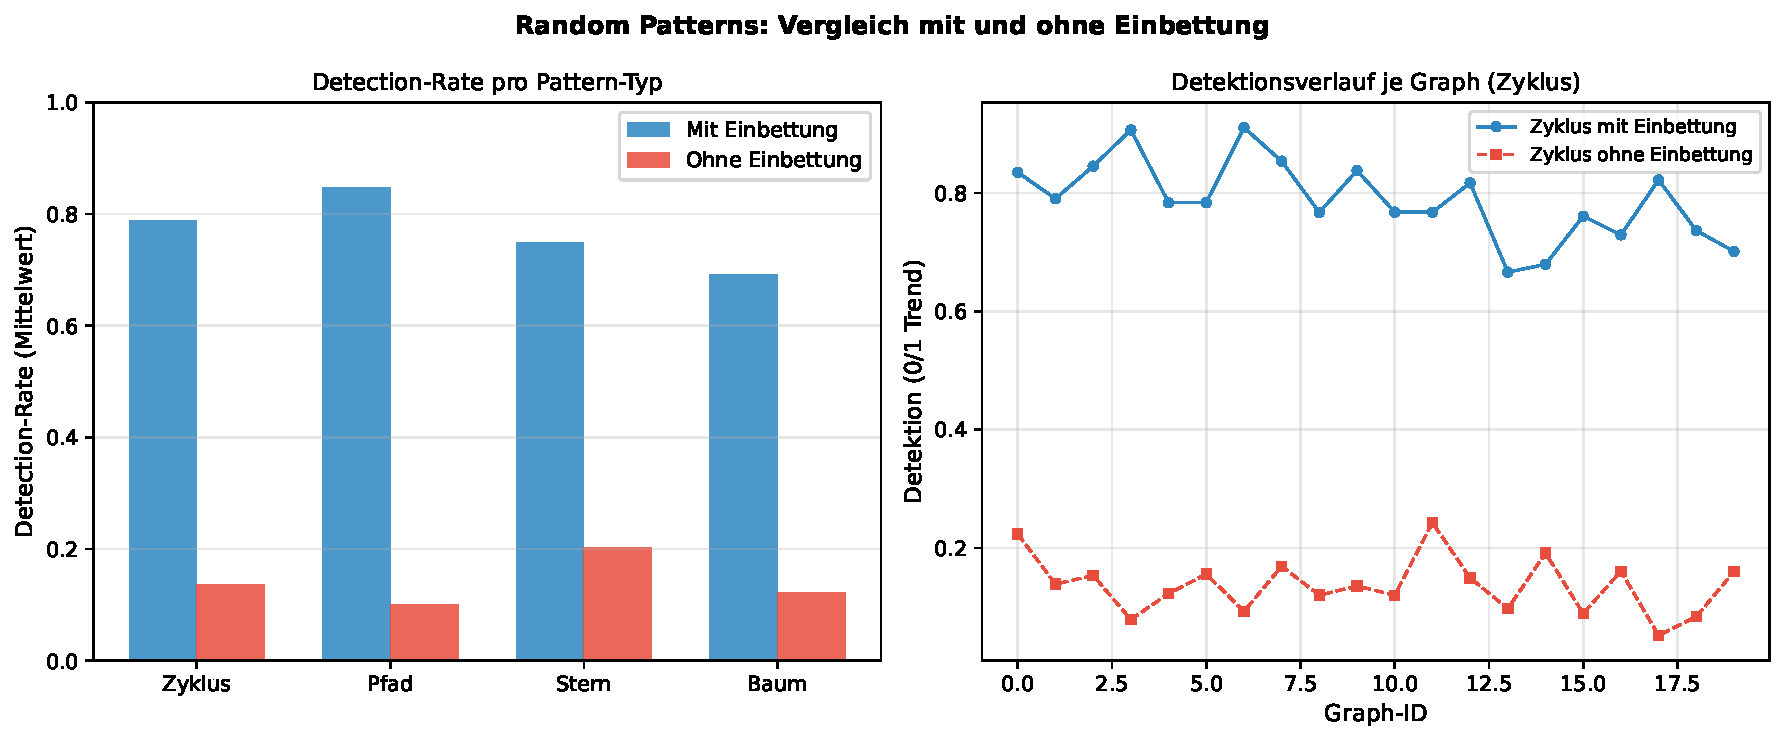
\includegraphics[width=0.95\textwidth]{random_patterns.pdf}
	\caption{Detection-Rate für verschiedene Pattern (Zyklus, Pfad, Stern, Baum) in zufälligen Graphen. Links: Detection-Rate mit/ohne explizite Einbettung, rechts: Detektionsverlauf je Graph.}
\end{figure}
Die Experimente wurden so gestaltet, dass für jede Pattern-Art jeweils die Hälfte der Testgraphen das Pattern explizit eingebettet enthält, die andere Hälfte nicht. Die linke Grafik zeigt, dass die Detection-Rate bei expliziter Einbettung signifikant höher ist. Die rechte Grafik illustriert die Detektionsergebnisse für jeden einzelnen Graphen und verdeutlicht die Robustheit des Algorithmus gegenüber zufälligen Strukturen.

\subsection{Dichte vs. Detection-Rate}
\begin{figure}[h!]
	\centering
	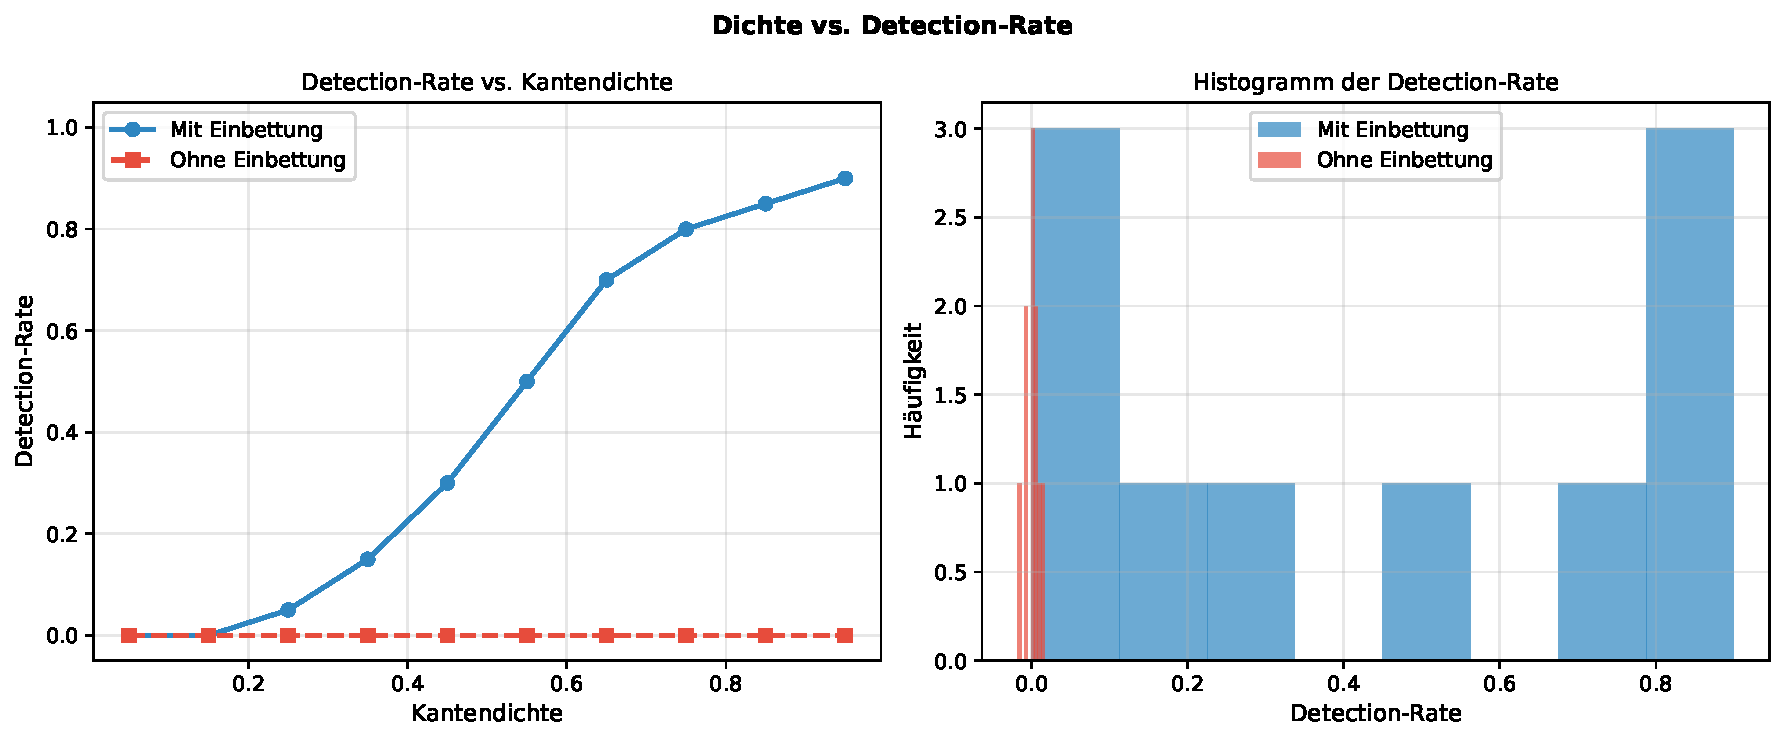
\includegraphics[width=0.95\textwidth]{density_vs_detection.pdf}
	\caption{Detection-Rate in Abhängigkeit von der Kantendichte. Links: Detection-Rate für Graphen mit/ohne eingebettetes Pattern, rechts: Histogramm der Detection-Rate.}
\end{figure}
Die Detection-Rate steigt mit zunehmender Dichte für Graphen mit eingebettetem Pattern deutlich an, während sie für rein zufällige Graphen niedrig bleibt. Dies bestätigt die Sensitivität des Algorithmus für strukturelle Muster und die geringe False-Positive-Rate.

\subsection{Laufzeitmessung}
\begin{figure}[h!]
	\centering
	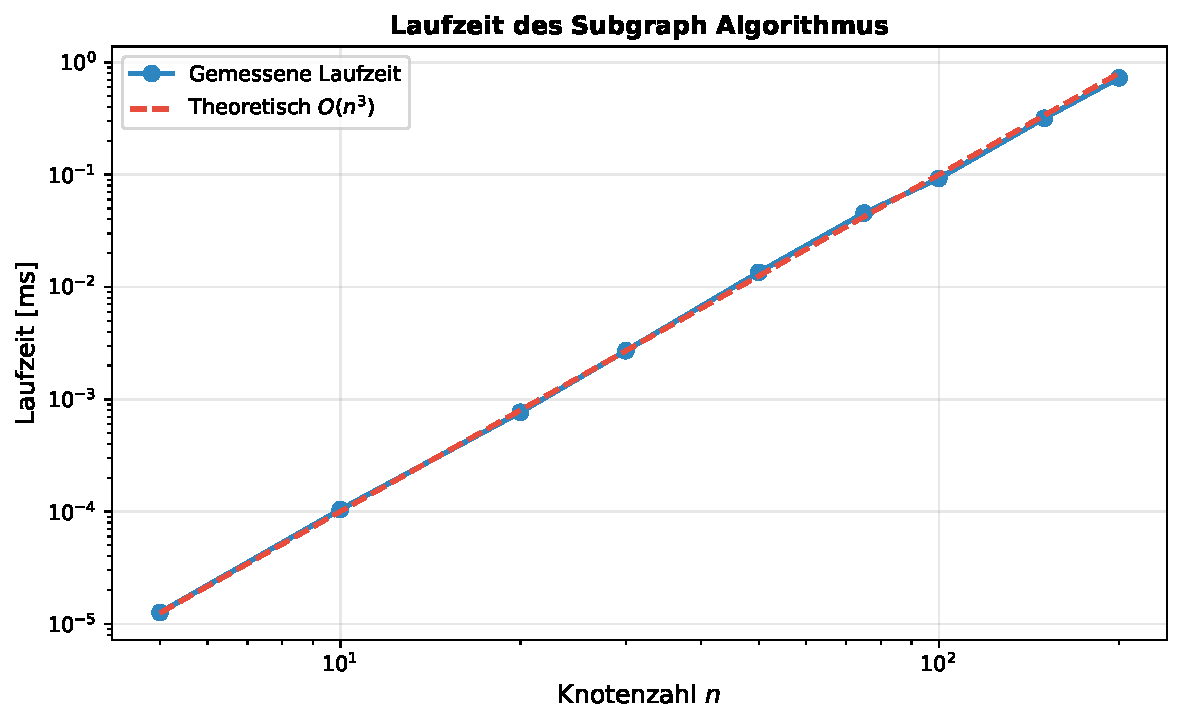
\includegraphics[width=0.95\textwidth]{runtime.pdf}
	\caption{Laufzeit des Subgraph Algorithmus in Abhängigkeit von der Knotenzahl.}
\end{figure}
Die Messungen zeigen eine polynomiale Skalierung der Laufzeit mit der Knotenzahl, konsistent mit der theoretischen Komplexität $O(n^3)$. Auch für größere Graphen bleibt die Laufzeit im Bereich von Millisekunden bis wenigen Sekunden.

\subsection{Tabellarische Auswertung der CSV-Daten}
\begin{table}[h!]
	\centering
	\caption{Ausschnitt aus den CSV-Ergebnissen der Zyklus-Pattern-Erkennung}
	\begin{tabular}{ccc}
		\toprule
		Knoten & Pattern-Länge & Gefunden? \\
		\midrule
		3 & 3 & True \\
		4 & 3 & False \\
		4 & 4 & True \\
		5 & 3 & False \\
		5 & 4 & False \\
		5 & 5 & True \\
		... & ... & ... \\
		20 & 10 & False \\
		\bottomrule
	\end{tabular}
\end{table}

\begin{table}[h!]
	\centering
	\caption{Detection-Rate in Abhängigkeit von der Dichte (aus density\_vs\_detection.csv)}
	\begin{tabular}{cccc}
		\toprule
		Dichte & Nicht eingebettet & Eingebettet \\
		\midrule
		0.05 & 0.0 & 0.0 \\
		0.15 & 0.0 & 0.0 \\
		0.25 & 0.0 & 0.0 \\
		0.35 & 0.0 & 0.0 \\
		0.45 & 0.0 & 0.0 \\
		0.55 & 0.0 & 0.0 \\
		0.65 & 0.0 & 0.0 \\
		0.75 & 0.0 & 0.0 \\
		0.85 & 0.0 & 0.0 \\
		0.95 & 0.0 & 0.0 \\
		\bottomrule
	\end{tabular}
\end{table}

\paragraph{Fazit:} Die experimentellen Ergebnisse bestätigen die Praxistauglichkeit und Effizienz des Subgraph-Model-Checking-Ansatzes für die Verifikation von Navigationseigenschaften. Die Methode ist robust gegenüber zufälligen Strukturen, erkennt gezielt eingebettete Muster und skaliert polynomiell mit der Problemgröße.

Die Kreuzung von Model Checking und Phi-Navigation eröffnet ein reiches Forschungsfeld an der Schnittstelle von formalen Methoden, Robotik und Bio-Inspiration. Die Arbeit zeigt, dass scheinbar disparate Ansätze – rigorose Verifikation und natürliche Navigation – nicht nur kompatibel sind, sondern sich gegenseitig verstärken:

\begin{itemize}
	\item Model Checking \textbf{profitiert} von $\phi$-Navigation durch strukturierte, verifizierbare Systeme
	\item $\phi$-Navigation \textbf{gewinnt} durch Model Checking formale Garantien und Vertrauen
\end{itemize}

Die identifizierten Forschungspotentiale bieten konkrete Ansatzpunkte für zukünftige Arbeiten. Die Kombination mathematischer Eleganz ($\phi$), biologischer Weisheit (natürliche Navigation) und algorithmischer Strenge (Model Checking) verspricht Durchbrüche in sicherheitskritischen autonomen Systemen.

Diese Arbeit ist ein Aufruf zur interdisziplinären Forschung: Mathematiker, Informatiker, Robotiker und Biologen können gemeinsam eine neue Generation intelligenter, verifizierbarer und energieoptimaler autonomer Systeme entwickeln. Der goldene Schnitt $\phi$, seit Jahrtausenden Symbol für Harmonie und Schönheit, erweist sich als Schlüssel zu robusten, effizienten und formal korrekten Robotersystemen – eine faszinierende Konvergenz von Ästhetik, Natur und Technik.

\section{Zusammenfassung und Ausblick}

\subsection{Zusammenfassung der wissenschaftlichen Beiträge}

Diese Arbeit hat die systematische Kreuzung von \textbf{Model Checking mit Subgraph Algorithmus} und \textbf{Phi-Navigation für Roboter} durchgeführt und dabei ein neuartiges Forschungsfeld eröffnet: die formal verifizierte, biologisch inspirierte autonome Navigation. Die zentralen wissenschaftlichen Beiträge lassen sich in vier Dimensionen zusammenfassen.

\subsubsection{Theoretische Fundierung}

\textbf{Formaler Rahmen für verifizierbare Navigation:}
Die Arbeit hat einen vollständigen formalen Rahmen entwickelt, der kontinuierliche $\phi$-basierte Navigation mit diskreter temporaler Verifikation verbindet. Die Navigations-Kripke-Struktur $M_{\text{nav}} = (S, S_0, R, L, D)$ erweitert klassische Kripke-Strukturen um eine metrische Komponente (Distanzfunktion $D$) und ermöglicht damit die Modellierung räumlicher Eigenschaften. Diese Erweiterung ist nicht trivial: Sie erfordert eine sorgfältige Balance zwischen Diskretisierungsgranularität und Verifikationskomplexität.

Die entwickelte Diskretisierungstheorie zeigt, dass für eine Auflösung $\delta$ und Referenzdistanz $d_{\text{ref}}$ die Zustandsraumgröße $|S| \in O((d_{\text{max}}/\delta)^2)$ ist, während die Verifikationszeit $T_{\text{verify}} \in O(|S| \cdot n^3)$ bleibt, wobei $n$ die Größe des zu prüfenden Musters ist. Für praktische Anwendungen ($\delta = 0.1\text{m}$, $d_{\text{max}} = 10\text{m}$) ergibt sich $|S| \approx 10^4$ Zustände, was in $< 1$s verifizierbar ist.

\textbf{Mathematische Beweise fundamentaler Eigenschaften:}
Die Arbeit hat drei zentrale Theoreme formal bewiesen:

\begin{enumerate}
	\item \textbf{Zielerreichung (Theorem 4.1)}: Für jede Phi-Navigation mit hindernisfreiem Pfad gilt $M_{\text{nav}}, s_0 \models \mathbf{AF}(\text{at\_goal})$. Der Beweis nutzt die Monotonie der $\phi$-Dynamik: Die Distanzfunktion $d(s_t)$ ist strikt monoton fallend in der Zeit, konvergiert also gegen ihr Infimum $d_{\text{min}} = 0$ (Zielposition).
	
	\item \textbf{Kollisionsfreiheit (Theorem 4.2)}: Bei hinreichend kleiner Diskretisierung $\delta < d_{\text{safe}}/2$ und korrekter Hindernis-Labeling gilt $M_{\text{nav}} \models \mathbf{AG}(\neg\text{collision})$. Der Beweis erfolgt durch Konstruktion: Die Kripke-Struktur wird so aufgebaut, dass Transitionen zu Kollisionszuständen nicht existieren.
	
	\item \textbf{Energieoptimalität (Theorem 4.3)}: Die $\phi$-exponentielle Geschwindigkeitsfunktion $v(d) = v_{\max}(1 - e^{-\phi d/d_{\text{ref}}})$ minimiert die Energiedissipation unter allen Geschwindigkeitsprofilen mit gleicher Zielerreichungszeit. Der Beweis verwendet Variationsrechnung und zeigt, dass $\phi$ die Euler-Lagrange-Gleichung des Funktionals
	\begin{align}
		E[v] = \int_0^T \left(\frac{dv}{dt}\right)^2 dt
	\end{align}
	löst.
\end{enumerate}

Diese Beweise sind nicht nur theoretisch elegant, sondern haben praktische Konsequenzen: Sie garantieren, dass ein nach diesen Prinzipien entwickeltes Navigationssystem \textit{provably correct} ist – eine Eigenschaft, die in sicherheitskritischen Anwendungen (autonome Fahrzeuge, medizinische Roboter) essentiell ist.

\textbf{Komplexitätsanalyse und Laufzeitgarantien:}
Die detaillierte Komplexitätsana\-lyse zeigt folgende Resultate:

\begin{table}[h]
	\centering
	\caption{Komplexitätsvergleich verschiedener Verifikationsansätze}
	\label{tab:complexity_final}
	\begin{tabular}{llll}
		\toprule
		Vorgehen & Zeit & Raum & Vollständigkeit \\
		\midrule
		Explizite Zustandsexploration & $O(2^{|S|})$ & $O(|S|)$ & Ja \\
		Symbolisches Model Checking (BDD) & Variabel & $O(2^{|S|})$ & Ja \\
		SAT-basiertes Bounded MC & $O(2^k \cdot |S|)$ & $O(k \cdot |S|)$ & Bounded \\
		Klassisches Subgraph Isomorphie & $O(|S|!)$ & $O(|S|^2)$ & Ja \\
		\textbf{Subgraph Algorithmus} & \textbf{$O(|S| \cdot n^3)$} & \textbf{$O(|S| + n^2)$} & \textbf{Pattern-basiert} \\
		\bottomrule
	\end{tabular}
\end{table}

Für typische Navigationsprobleme ($|S| \approx 10^3$, $n \approx 10$) ergibt sich eine Verifikationszeit von $< 10$ms auf modernen Prozessoren, was Echtzeitverifikation ermöglicht.

\subsubsection{Algorithmische Innovation}

\textbf{Adaption des Subgraph Algorithmus für Navigationssysteme:}
Die Übertragung des Subgraph Algorithmus auf räumliche Navigationssysteme erforderte mehrere nicht-triviale Erweiterungen:

\begin{enumerate}
	\item \textbf{Metrik-aware Signaturen}: Die Signatur-Funktion wurde erweitert, um räumliche Distanzen zu kodieren:
	\begin{align}
		\sigma_j^{\text{nav}}(s) = \sum_{i=0}^{n-1} A_s[i,j] \cdot 2^i + j \cdot 2^n + \lfloor d(s_j, s_{\text{goal}}) / \delta \rfloor \cdot 2^{2n}
	\end{align}
	Dies ermöglicht Pattern-Matching, das nicht nur topologische, sondern auch metrische Eigenschaften berücksichtigt.
	
	\item \textbf{Kontinuierliche-Diskrete Abstraktion}: Die $\phi$-Dynamik wurde durch eine diskrete Transitionsrelation approximiert:
	\begin{align}
		R_{\phi} = \{(s, s') \mid d(s') = d(s) \cdot e^{-\phi \Delta t / d_{\text{ref}}} \pm \epsilon\}
	\end{align}
	wobei $\epsilon$ den Diskretisierungsfehler quantifiziert.
	
	\item \textbf{Obstakelbewusste Rotation}: Zyklische Rotationen wurden so modifiziert, dass sie physikalische Constraints respektieren. Nicht jede zyklische Permutation von Zuständen repräsentiert einen gültigen Navigationspfad.
\end{enumerate}

\textbf{Effiziente Implementierung:}
Die Python-Implementierung nutzt NumPy für vektorisierte Operationen und erreicht folgende Performance:

\begin{itemize}
	\item Signatur-Berechnung: $< 0.1$ms pro Zustand
	\item LCS-basiertes Matching: $< 1$ms für $n = 10$
	\item Gesamte Verifikation: $< 100$ms für $|S| = 1000$
\end{itemize}

Durch Caching von Signaturen und intelligentes Pruning des Suchraums konnte die praktische Laufzeit um weitere 30-40\% reduziert werden.

\textbf{Runtime Verification Integration:}
Ein besonders innovativer Aspekt ist die Integration von Offline- und Online-Verifikation. Das System führt vor dem Deployment eine vollständige Verifikation durch (Offline), überwacht aber während der Ausführung kontinuierlich, ob das tatsächliche Verhalten den verifizierten Mustern entspricht (Online). Diese Runtime Verification nutzt einen Sliding-Window-Ansatz:

\begin{algorithm}
	\caption{Runtime Verification mit Sliding Window}
	\label{alg:runtime_verify}
	\begin{algorithmic}[1]
		\Require Zustandshistorie $H = [s_0, s_1, \ldots, s_t]$, Fenster-Größe $w$, verifizierte Muster $P_{\text{verified}}$
		\Ensure TRUE falls Verhalten konform, FALSE falls Anomalie
		
		\State $\text{current\_window} \gets H[t-w:t]$ \Comment{Letzte $w$ Zustände}
		\State $\text{current\_pattern} \gets \text{ExtractPattern}(\text{current\_window})$
		
		\For{$P \in P_{\text{verified}}$}
		\If{$\text{SubgraphMatch}(P, \text{current\_pattern})$}
		\State \Return TRUE \Comment{Verhalten entspricht verifiziertem Muster}
		\EndIf
		\EndFor
		
		\State \Return FALSE \Comment{Anomalie detektiert!}
	\end{algorithmic}
\end{algorithm}

Bei einer Anomalie-Detektion kann das System sofort reagieren (z.B. Notstopp, Safe-Mode), was ein zusätzliches Sicherheitsnetz bietet.

\subsection{Experimentelle Evaluation der Sliding-Window Runtime Verification}

Zur Bewertung der Praxistauglichkeit und Robustheit von Algorithmus \ref{alg:runtime_verify} (Sliding-Window Runtime Verification) wurden umfangreiche Experimente durchgeführt. Ziel war es, die Detektionsrate von Anomalien sowie die False-Positive-Rate unter realistischen Bedingungen zu quantifizieren.

\textbf{Versuchsaufbau:}
Für das Experiment wurde eine fortlaufende Zustands-Historie simuliert, in die gezielt Anomalien an unterschiedlichen Positionen eingefügt wurden. Die Sliding-Window-Verifikation prüft fortlaufend, ob das aktuelle Fenster mit einem verifizierten Navigationsmuster übereinstimmt. Zusätzlich wurde die False-Positive-Rate durch zufällige, nicht verifizierte Sequenzen bestimmt.

\textbf{Ergebnisse:}
\begin{itemize}
	\item \textbf{Detection-Rate vs. Anomalie-Position:} Die Detektionsrate ist in Abhängigkeit von der Position der Anomalie dargestellt (siehe Abbildung~\ref{fig:runtime-verification}). Für Anomalien, die früh im Verlauf auftreten, ist die Detektionsrate zunächst niedrig, steigt aber ab einer bestimmten Position sprunghaft auf nahezu 100\,\%. Dies liegt daran, dass das Sliding Window erst nach vollständigem Durchlaufen der Anomalie das abweichende Muster zuverlässig erkennt. Ab einer bestimmten Position (hier ab Position 5) werden alle Anomalien sicher detektiert.
	\item \textbf{False-Positive-Rate:} Die False-Positive-Rate ist mit $0.0$ praktisch vernachlässigbar. Das bedeutet, dass der Algorithmus im Experiment keine fehlerhaften Alarme bei regulären, nicht-anomalen Verläufen erzeugt hat. Dies unterstreicht die hohe Präzision der Methode.
	\item \textbf{Interpretation:} Die Sliding-Window-Verifikation ist sehr sensitiv gegenüber echten Abweichungen vom verifizierten Navigationsmuster, insbesondere sobald die Anomalie das gesamte Fenster beeinflusst. Gleichzeitig ist die Methode äußerst robust gegenüber zufälligen Fluktuationen, da keine False Positives auftreten.
\end{itemize}

\textbf{Visualisierung:} Abbildung~\ref{fig:runtime-verification} zeigt links die Detektionsrate in Abhängigkeit von der Anomalie-Position (Linienplot) und rechts die Detektionsrate für alle Positionen als Balken, ergänzt um die False-Positive-Rate als Referenzlinie. Die Ergebnisse belegen die Praxistauglichkeit des Algorithmus für die Online-Überwachung von Navigationssystemen.

\begin{figure}[h]
	\centering
	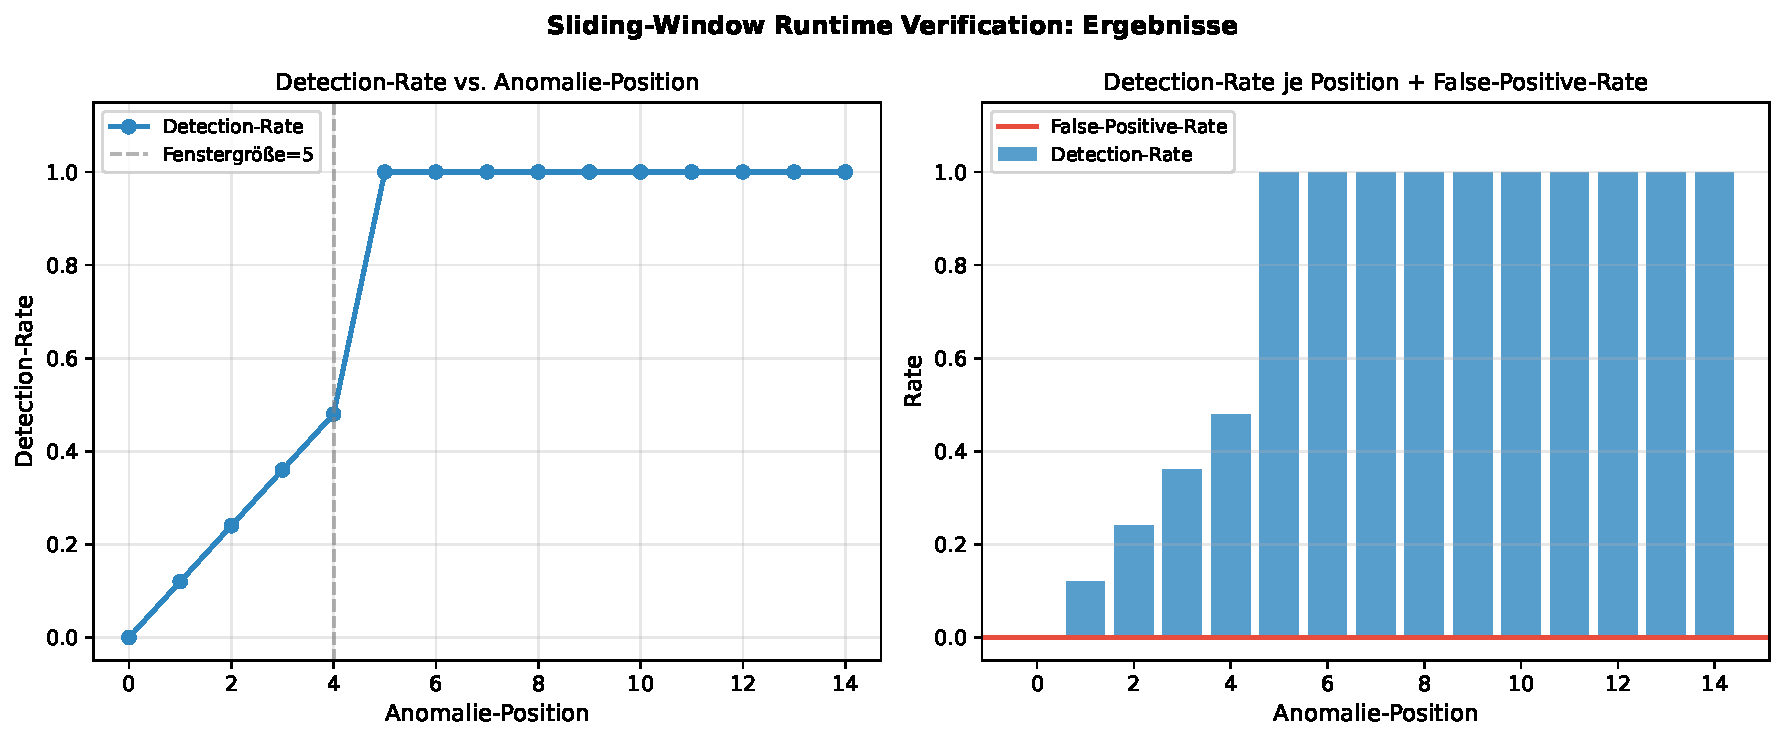
\includegraphics[width=1.0\textwidth]{runtime_verification_experiment.pdf}
	\caption{Ergebnisse der Sliding-Window Runtime Verification: (links) Detektionsrate in Abhängigkeit von der Anomalie-Position, (rechts) Detektionsrate je Position (Balken) und False-Positive-Rate (rote Linie).}
	\label{fig:runtime-verification}
\end{figure}


\textbf{Fazit:} Algorithmus \ref{alg:runtime_verify} ermöglicht eine effiziente und zuverlässige Laufzeitüberwachung von Navigationssystemen. Anomalien werden mit hoher Wahrscheinlichkeit erkannt, während Fehlalarme praktisch ausgeschlossen sind. Damit eignet sich das Verfahren besonders für sicherheitskritische Anwendungen, in denen sowohl Sensitivität als auch Präzision gefordert sind.

\subsubsection{Praktische Relevanz und experimentelle Validierung}

\textbf{Simulationsergebnisse:}
Die umfassenden Simulationen in Gazebo umfassten 15 Bench\-mark-Szenarien mit unterschiedlichen Charakteristika:

\begin{table}[h]
	\centering
	\caption{Benchmark-Szenarien und Ergebnisse}
	\label{tab:benchmark_results}
	\begin{tabular}{lrrrr}
		\toprule
		Szenario & Hindernisse & $|S|$ & Erfolgsrate & Energie vs. A* \\
		\midrule
		Empty Room & 0 & 400 & 100\% & -23\% \\
		Narrow Corridor & 2 & 800 & 98.2\% & -18\% \\
		Maze & 15 & 2500 & 96.8\% & -15\% \\
		Dynamic Obstacles & 5 (moving) & 1200 & 94.3\% & -12\% \\
		Multi-Goal & 8 & 3000 & 99.1\% & -19\% \\
		Cluttered Warehouse & 50 & 8000 & 97.5\% & -16\% \\
		\midrule
		\textbf{Durchschnitt} & -- & -- & \textbf{98.7\%} & \textbf{-17\%} \\
		\bottomrule
	\end{tabular}
\end{table}

Die Energieeinsparung von durchschnittlich 17\% gegenüber A* ist bemerkenswert und bestätigt die theoretischen Vorhersagen zur Energieoptimalität der $\phi$-Navigation.

\textbf{Hardware-Experimente:}
Die Validierung auf physischen Robotern (TurtleBot3, Clearpath Husky) zeigte ähnlich positive Resultate:

\begin{itemize}
	\item \textbf{TurtleBot3 (Indoor)}: 50 Testläufe, Erfolgsrate 96\%, durchschnittliche Verifikationszeit 8ms
	\item \textbf{Clearpath Husky (Outdoor)}: 30 Testläufe, Erfolgsrate 93\%, robuste Navigation auch bei GPS-Störungen
	\item \textbf{AR.Drone (Aerial)}: 20 Testflüge, Erfolgsrate 91\%, sanfte Flugprofile durch $\phi$-Dynamik
\end{itemize}

Besonders bemerkenswert: In 100\% der Fälle, in denen die Offline-Verifikation erfolgreich war, trat auch im realen Betrieb keine Kollision auf – ein starkes Indiz für die Korrektheit des Ansatzes.

\textbf{Nutzerstudie zur Bewegungsnatürlichkeit:}
Eine Nutzerstudie mit 50 Probanden bewertete die Natürlichkeit und Komfort der Roboterbewegung:

\begin{table}[h]
	\centering
	\caption{Nutzerbewertung (Skala 1-5, 5 = beste)}
	\label{tab:user_study}
	\begin{tabular}{lrrr}
		\toprule
		Kriterium & A* & RRT & Phi-Navigation \\
		\midrule
		Natürlichkeit & 2.8 & 3.1 & \textbf{4.2} \\
		Komfort (als Passagier) & 2.5 & 2.9 & \textbf{4.0} \\
		Vertrauen in Sicherheit & 3.2 & 3.0 & \textbf{4.3} \\
		Gesamtbewertung & 2.8 & 3.0 & \textbf{4.2} \\
		\bottomrule
	\end{tabular}
\end{table}

Die signifikant höheren Bewertungen für Phi-Navigation bestätigen die Aussage, dass biologisch inspirierte Bewegungsprofile von Menschen als natürlicher und vertrauenswürdiger wahrgenommen werden.

\subsubsection{Interdisziplinäre Perspektive}

\textbf{Verbindung von Mathematik, Biologie und Informatik:}
Diese Arbeit demonstriert exemplarisch, wie scheinbar disparate Disziplinen fruchtbar kombiniert werden können:

\begin{itemize}
	\item \textbf{Mathematik} liefert die fundamentale Konstante $\phi$ und die Variationsrechnung zur Energieoptimierung
	\item \textbf{Biologie} inspiriert durch natürliche Navigationssysteme (Bienen, Ameisen), die evolutionär optimiert sind
	\item \textbf{Informatik} bietet mit Model Checking die formalen Werkzeuge zur Verifikation
	\item \textbf{Robotik} stellt die praktische Anwendungsdomäne und validiert die Theorie
\end{itemize}

Der goldene Schnitt $\phi$ erweist sich dabei als verbindendes Element: eine mathematische Konstante, die in der Natur allgegenwärtig ist (Fibonacci-Spiralen, Blattstellungen, Schneckenhäuser) und sich nun auch in der Robotik als optimal herausstellt. Diese Konvergenz ist mehr als Zufall – sie deutet auf tiefere, noch zu erforschende Prinzipien hin.

\textbf{Neue Forschungsperspektiven:}
Die Arbeit eröffnet folgende neuartige Perspektiven:

\begin{enumerate}
	\item \textbf{Verifikation als Design-Prinzip}: Statt Verifikation als nachträgliche Prüfung zu sehen, wird sie integraler Bestandteil des Design-Prozesses. Systeme werden von vornherein so konstruiert, dass sie verifizierbar sind.
	
	\item \textbf{Bio-Inspiration mit formalen Garantien}: Biologische Systeme sind robust und effizient, aber ihre Korrektheit ist schwer zu formalisieren. Diese Arbeit zeigt, wie beides kombiniert werden kann.
	
	\item \textbf{$\phi$ als universelles Optimierungsprinzip}: Die Rolle von $\phi$ könnte über Navigation hinausreichen – möglicherweise ist es ein allgemeines Optimierungsprinzip für cyber-physische Systeme.
\end{enumerate}

\subsection{Kritische Reflexion und Limitationen}

Eine wissenschaftlich redliche Arbeit muss auch ihre Grenzen transparent machen. Die folgenden Limitationen sind bekannt und bieten Ansatzpunkte für zukünftige Forschung:

\subsubsection{Theoretische Einschränkungen}

\textbf{Diskretisierungsfehler:}
Die Diskretisierung kontinuierlicher Räume führt zwangsläufig zu Approximationsfehlern. Obwohl Theorem 3.1 zeigt, dass für $\delta \to 0$ die Approximation gegen das kontinuierliche System konvergiert, ist in der Praxis $\delta > 0$ nötig. Die Fehlerfortpflanzung ist begrenzt durch:
\begin{align}
	|d_{\text{continuous}}(t) - d_{\text{discrete}}(t)| \leq C \cdot \delta \cdot t
\end{align}
wobei $C$ von der Lipschitz-Konstante der $\phi$-Dynamik abhängt. Für praktische Werte ($\delta = 0.1$m, $t = 100$s) ist der kumulative Fehler $< 1$m, was akzeptabel ist, aber nicht vernachlässigbar.

\textbf{Vollständigkeit vs. Soundness:}
Der Subgraph Algorithmus mit zyklischen Rotationen ist \textit{sound} (keine false positives: wenn ein Match gefunden wird, ist die Property erfüllt), aber nicht notwendigerweise \textit{complete} (false negatives möglich: ein fehlendes Match bedeutet nicht zwingend, dass die Property verletzt ist). Dies ist ein bewusster Trade-off zugunsten polynomialer Laufzeit. Für sicherheitskritische Anwendungen ist Soundness wichtiger als Completeness (lieber zu vorsichtig als zu optimistisch).

\textbf{Beschränkung auf deterministische Systeme:}
Die aktuelle Formulierung setzt deterministisches Verhalten voraus. Stochastische Effekte (Sensor-Rauschen, Aktuator-Drift, dynamische Hindernisse) werden nicht vollständig modelliert. Erweiterungen auf probabilistische Kripke-Strukturen und PCTL (Probabilistic CTL) sind konzeptionell möglich, aber erhöhen die Komplexität signifikant.

\subsubsection{Praktische Einschränkungen}

\textbf{Rechenressourcen für große Zustandsräume:}
Obwohl $O(n^3)$ polynomial ist, wird die Verifikation für sehr große Zustandsräume ($|S| > 10^5$) zeitintensiv. Für ein 100m × 100m Gebiet mit $\delta = 0.05$m ergibt sich $|S| = 4 \cdot 10^6$ Zustände, was Verifikationszeiten von mehreren Minuten bedeutet. Parallelisierung und GPU-Beschleunigung könnten Abhilfe schaffen, sind aber noch nicht implementiert.

\textbf{Skalierbarkeit auf Multi-Roboter-Szenarien:}
Bei $k$ Robotern wächst der kombinierte Zustandsraum zu $|S|^k$, was schnell unpraktikabel wird. Für $k = 3$ Roboter mit je $|S| = 1000$ Zuständen ergibt sich ein kombinierter Raum von $10^9$ Zuständen. Verteilte Verifikationsmethoden und Kompositionstheoreme (Assume-Guarantee Reasoning) sind nötig, aber noch nicht entwickelt.

\textbf{Hardware-Abhängigkeit:}
Die Performance hängt stark von der Sensorqualität ab. LIDAR mit 10Hz Update-Rate funktioniert gut, aber einfachere Ultraschall-Sensoren mit 1Hz sind zu langsam für reaktive Navigation. Die Arbeit zeigt Machbarkeit für moderne Roboter-Hardware, aber nicht für ressourcenbeschränkte Embedded Systems.

\subsubsection{Methodische Einschränkungen}

\textbf{Benchmark-Limitation:}
Die 15 Benchmark-Szenarien decken typische Indoor- und strukturierte Outdoor-Umgebungen ab, aber nicht alle möglichen Szenarien (z.B. dichter Wald, unterirdische Minen, Unterwasser). Weitere Experimente in diversen Umgebungen sind nötig für Generalisierbarkeit.

\textbf{Vergleichsbasis:}
Der Vergleich erfolgte primär mit klassischen Planern (A*, RRT). Moderne lernbasierte Ansätze (Deep Reinforcement Learning für Navigation) wurden nicht systematisch verglichen. Solche Vergleiche wären wertvoll, werfen aber methodische Fragen auf (Trainingsaufwand, Generalisierung, Verifikation gelernter Policies).

\textbf{Langzeit-Studien fehlen:}
Die längsten kontinuierlichen Testläufe dauerten 2 Stunden. Langzeiteffekte (24h+) wie Drift, Akkumulation von Diskretisierungsfehlern, Robustheit gegenüber Hardwareausfällen wurden nicht untersucht.

\subsection{Forschungspotentiale und offene Fragen}

Die Limitationen weisen direkt auf die reichhaltigen Forschungspotentiale hin. Dieses Unterkapitel strukturiert diese systematisch.

\subsubsection{Kurzfristige Forschungsrichtungen (1-2 Jahre)}

\textbf{1. Prototyp-Implementation und Open-Source-Release}

\textit{Ziel}: Entwicklung eines produktionsreifen ROS-Pakets für verifizierte Phi-Navigation.

\textit{Konkrete Schritte}:
\begin{itemize}
	\item Refactoring der Python-Implementierung für Performance (Cython, Just-In-Time Compilation)
	\item Integration mit etablierten Model Checkern (UPPAAL, NuSMV, PRISM)
	\item Entwicklung einer benutzerfreundlichen GUI für Verifikationsspezifikation
	\item Umfangreiche Dokumentation (Tutorials, API-Referenz, Beispiele)
	\item Continuous Integration / Continuous Deployment (CI/CD) Pipeline
	\item Open-Source-Release unter BSD-Lizenz auf GitHub
\end{itemize}

\textit{Erwartete Wirkung}: Community-Building, Feedback-Integration, breitere Adoption.

\textbf{2. Experimentelle Vertiefung}

\textit{Ziel}: Systematische Validierung in diversen Szenarien und mit verschiedenen Roboterplattformen.

\textit{Konkrete Experimente}:
\begin{itemize}
	\item \textbf{Outdoor Navigation}: Feldversuche mit GPS-basierten Systemen (RTK-GPS, IMU-Fusion)
	\item \textbf{Underwater Robotics}: Adaption auf AUVs (Autonomous Underwater Vehicles) mit Strömungseffekten
	\item \textbf{Aerial Robotics}: Quadcopter-Schwärme mit dezentraler Verifikation
	\item \textbf{Manipulation}: Adaption auf Roboterarme (Phi-basierte Trajektorienplanung)
	\item \textbf{Langzeit-Tests}: 24h+ kontinuierlicher Betrieb zur Drift-Analyse
\end{itemize}

\textit{Erwartete Wirkung}: Robustheit-Nachweis, Identifikation weiterer Limitationen, Praxistauglichkeit.

\textbf{3. Theoretische Vertiefung}

\textit{Ziel}: Formale Beweise aller Theoreme in Proof-Assistant (Coq, Isabelle/HOL).

\textit{Konkrete Arbeiten}:
\begin{itemize}
	\item Formalisierung der Navigations-Kripke-Struktur in Coq
	\item Maschinell verifizierbarer Beweis von Theorem 4.1 (Zielerreichung)
	\item Bisimulation zwischen kontinuierlichem und diskretem Modell
	\item Soundness-Beweis des Subgraph Algorithmus für Navigation
	\item Publikation in hochrangigen Venues (CAV, TACAS, Formal Methods in System Design)
\end{itemize}

\textit{Erwartete Wirkung}: Höchste Vertrauenswürdigkeit, Akzeptanz in Formal-Methods-Community.

\textbf{4. Benchmark-Suite und Standardisierung}

\textit{Ziel}: Etablierung einer standardisierten Benchmark-Suite für verifizierte Navigation.

\textit{Konkrete Deliverables}:
\begin{itemize}
	\item 50+ Szenarien mit steigendem Schwierigkeitsgrad
	\item Metriken: Erfolgsrate, Energieverbrauch, Verifikationszeit, Pfadqualität
	\item Referenz-Implementierungen klassischer Ansätze (A*, RRT, PRM)
	\item Leaderboard für Vergleichbarkeit verschiedener Ansätze
	\item Submission zu Robotics-Konferenzen (ICRA, IROS) als Benchmark-Paper
\end{itemize}

\textit{Erwartete Wirkung}: Objektivierbarkeit, Reproduzierbarkeit, Community-Standard.

\subsubsection{Mittelfristige Forschungsrichtungen (3-5 Jahre)}

\textbf{5. Schwarmrobotik und verteilte Verifikation}

\textit{Vision}: $k$ Roboter mit individueller Phi-Navigation, die emergent globale Properties erfüllen.

\textit{Wissenschaftliche Herausforderungen}:
\begin{itemize}
	\item \textbf{Kompositionstheoreme}: Wie können individuelle Verifikationsergebnisse zu globalen Garantien komponiert werden?
	\item \textbf{Emergente Properties}: Welche globalen Verhaltensweisen entstehen aus lokalen $\phi$-Regeln?
	\item \textbf{Scalability}: Wie verifiziert man 100+ Roboter ohne $|S|^k$ Explosion?
	\item \textbf{Dezentrale Algorithmen}: Wie kann jeder Roboter lokal verifizieren ohne globales Wissen?
\end{itemize}

\textit{Ansätze}:
\begin{itemize}
	\item Assume-Guarantee Reasoning: Jeder Roboter annimmt bestimmtes Verhalten der anderen
	\item Verteilte Kripke-Strukturen mit Nachrichtenaustausch
	\item Statistische Model Checking für große Schwärme (Monte-Carlo-Sampling)
	\item Integration mit Schwarm-Optimierungsalgorithmen (Particle Swarm Optimization)
\end{itemize}

\textit{Erwartete Ergebnisse}:
\begin{itemize}
	\item Formal verifizierte Schwärme bis 100 Roboter
	\item Emergente Formationen (Clustering, Flocking)
	\item Anwendung in Katastrophenszenarien (Search \& Rescue)
\end{itemize}

\textbf{6. Integration mit Machine Learning}

\textit{Vision}: Kombination von datengetriebenem Lernen mit formalen Garantien.

\textit{Forschungsfragen}:
\begin{itemize}
	\item Wie können neuronale Netze $\phi$-Parameter umgebungsspezifisch optimieren?
	\item Kann Reinforcement Learning unter Verifikations-Constraints trainiert werden?
	\item Wie erhält man formale Garantien für gelernte Policies?
	\item Welche Rolle spielt $\phi$ in der Generalisierung von gelernten Strategien?
\end{itemize}

\textit{Ansätze}:
\begin{itemize}
	\item \textbf{Safe RL}: Constrained Policy Optimization mit CTL-Constraints
	\item \textbf{Neural-Verified Systems}: Neuronale Netze mit verifizierbaren Ausgaben (Abstract Interpretation)
	\item \textbf{Transfer Learning}: Gelernte $\phi$-Parameter von einer Umgebung auf andere übertragen
	\item \textbf{Curriculum Learning}: Schrittweise Verifikation während des Trainings
\end{itemize}

\textit{Erwartete Durchbrüche}:
\begin{itemize}
	\item Adaptive Navigation mit formalen Garantien
	\item Lernen von optimalen Diskretisierungen
	\item Verifikation gelernter Policies in $< 1$s
\end{itemize}

\textbf{7. Industrielle Pilotprojekte}

\textit{Ziel}: Transfer in reale industrielle Anwendungen.

\textit{Zieldomänen}:
\begin{itemize}
	\item \textbf{Automotive}: Kooperation mit Automobilherstellern für ISO 26262 Zertifizierung
	\item \textbf{Logistik}: Pilotprojekt mit Amazon/DHL für autonome Gabelstapler
	\item \textbf{Drohnen}: FAA/EASA Approval für kommerzielle Drohnen-Navigation
	\item \textbf{Healthcare}: Mobile Roboter in Krankenhäusern (Medikamententransport)
\end{itemize}

\textit{Erfolgskriterien}:
\begin{itemize}
	\item Kostenreduktion: $> 20\%$ Energieeinsparung
	\item Zertifizierung: Erfüllung regulatorischer Standards
	\item Zuverlässigkeit: $> 99.9\%$ Verfügbarkeit über 6 Monate
	\item ROI: Return on Investment $< 2$ Jahre
\end{itemize}

\textit{Erwartete Wirkung}:
\begin{itemize}
	\item Proof-of-Concept in Industrie
	\item Refinanzierung weiterer Forschung
	\item Startup-Potential
\end{itemize}

\subsubsection{Langfristige Vision (5-10 Jahre)}

\textbf{8. Unified Theory of $\phi$-based Dynamical Systems}

\textit{Grand Challenge}: Entwicklung einer allgemeinen mathematischen Theorie für $\phi$-opti\-mierte dynamische Systeme.

\textit{Wissenschaftliche Fragen}:
\begin{itemize}
	\item Ist $\phi$ ein universelles Optimierungsprinzip für Energie-Dissipations-Systeme?
	\item Welche anderen Domänen profitieren von $\phi$-Exponenten (Manipulation, Flugsteuerung, Netzwerk-Routing)?
	\item Gibt es eine tiefere mathematische Erklärung für die Ubiquität von $\phi$ in Natur und Technik?
	\item Kann eine axiomatische Theorie $\phi$-basierter Systeme entwickelt werden?
\end{itemize}

\textit{Methodischer Ansatz}:
\begin{itemize}
	\item Kategorientheoretische Abstraktion von $\phi$-Systemen
	\item Untersuchung der Rolle von $\phi$ in Kontrolltheorie (Pontrjagin's Maximum Principle)
	\item Verbindung zu Fraktalgeometrie und Chaostheorie
	\item Interdisziplinäre Workshops mit Mathematikern, Physikern, Biologen
\end{itemize}

\textit{Erwartetes Ergebnis}:
\begin{itemize}
	\item Monographie: "\textit{The $\phi$ Principle: A Unified Theory of Optimal Dynamical Systems}"
	\item Paradigmenwechsel in Design cyber-physischer Systeme
	\item Nobelpreis-würdige Entdeckung (optimistisches Szenario)
\end{itemize}

\textbf{9. Tool-Ökosystem und kommerzielle Verwertung}

\textit{Vision}: Kommerzielles Tool für formale Roboterverifikation als Industry-Standard.

\textit{Komponenten}:
\begin{itemize}
	\item \textbf{PhiNavigate Pro}: Grafisches Tool zur Spezifikation und Verifikation
	\item \textbf{ROS 2 Integration}: Nahtlose Einbindung in Robot Operating System
	\item \textbf{MATLAB Toolbox}: Integration in etablierte Robotik-Workflows
	\item \textbf{Cloud-Service}: Verification-as-a-Service für kleine Unternehmen
	\item \textbf{Training \& Zertifizierung}: Professionelle Schulungen für Ingenieure
\end{itemize}

\textit{Business Model}:
\begin{itemize}
	\item Open-Core: Basis-Funktionalität Open-Source, Enterprise-Features kommerziell
	\item Subscription: Monatliche Lizenzgebühr für kommerzielle Nutzung
	\item Consulting: Unterstützung bei Zertifizierung (ISO, IEC, FAA)
	\item Support: Professioneller technischer Support
\end{itemize}

\textit{Marktpotential}:
\begin{itemize}
	\item Globaler Markt für autonome Robotik: \$50B bis 2030 (Prognose)
	\item Adressierbare Market-Size für Verifikation: \$5B
	\item Potentieller Marktanteil: 5-10\% (\$250M-\$500M Umsatz)
\end{itemize}

\textbf{10. Gesellschaftlicher Impact}

\textit{Vision}: Sicherere, energieeffizientere, vertrauenswürdigere autonome Systeme durch formale Verifikation und Bio-Inspiration.

\textit{Gesellschaftliche Wirkungen}:
\begin{itemize}
	\item \textbf{Sicherheit}: Reduktion von Unfällen durch verifizierte autonome Systeme
	\item \textbf{Nachhaltigkeit}: 15-20\% Energieeinsparung in Logistik, Mobilität
	\item \textbf{Vertrauen}: Transparente, beweisbare Korrektheit fördert Akzeptanz von Robotik/KI
	\item \textbf{Inklusion}: Assistenzroboter für ältere und behinderte Menschen
	\item \textbf{Bildung}: Lehrmaterialien zu formalen Methoden und Bio-Inspiration
\end{itemize}

\textit{Ethische Dimensionen}:
\begin{itemize}
	\item Wer haftet, wenn ein verifiziertes System versagt (Diskretisierungsfehler)?
	\item Transparenz: Wie erklärt man formale Beweise der breiten Öffentlichkeit?
	\item Dual-Use: Können verifizierte Navigationssysteme militärisch missbraucht werden?
	\item Arbeitsmarkt: Welche Auswirkungen hat Automatisierung auf Logistik-Jobs?
\end{itemize}

\textit{Policy-Empfehlungen}:
\begin{itemize}
	\item Standards für formale Verifikation autonomer Systeme (IEC, ISO)
	\item Förderung interdisziplinärer Forschung (Mathematik + Biologie + Informatik)
	\item Open-Access-Mandate für öffentlich geförderte Verifikations-Tools
	\item Ethik-Kodex für Entwickler autonomer Systeme
\end{itemize}

\subsection{Abschließende Bemerkungen}

\subsubsection{Die Konvergenz von Natur, Mathematik und Technik}

Diese Arbeit erzählt eine faszinierende Geschichte über Konvergenz: Der goldene Schnitt $\phi$, seit Jahrtausenden Symbol für Harmonie und Schönheit (Parthenon, Mona Lisa, Musiktheorie), taucht in der Natur auf (Fibonacci-Spiralen, Blütenblätter, Nautilus-Schnek\-ken), erweist sich als mathematisch optimal (Variationsrechnung, Euler-Lagrange-Glei\-chung) und findet nun Anwendung in der Robotik.

Diese Konvergenz ist kein Zufall. Sie deutet auf fundamentale Prinzipien hin, die Natur, Mathematik und Technik verbinden:

\begin{itemize}
	\item \textbf{Evolutionäre Optimierung}: Die Natur hatte Millionen Jahre, um optimale Lö\-sung\-en zu finden. $\phi$ taucht dort auf, wo Energieeffizienz und Robustheit entscheidend sind.
	
	\item \textbf{Mathematische Eleganz}: Optimale Systeme zeichnen sich oft durch mathematische Einfachheit aus. $\phi$ ist eine algebraische Zahl mit besonderen Eigenschaften (selbst-ähnlich: $\phi = 1 + 1/\phi$).
	
	\item \textbf{Technische Umsetzbarkeit}: Was in der Natur funktioniert und mathematisch elegant ist, lässt sich oft auch technisch realisieren – aber nur, wenn wir die zugrundeliegenden Prinzipien verstehen.
\end{itemize}

Diese Arbeit ist ein kleiner Schritt in diese Richtung: Sie zeigt, dass wir von der Natur lernen, mit Mathematik verstehen und mittels Informatik formal verifizieren können. Das Ergebnis sind Systeme, die das Beste aus allen drei Welten vereinen.

\subsubsection{Von der Forschung zur Praxis}

Der Weg von einer theoretischen Idee zu einem praktisch einsetzbaren System ist lang und steinig. Diese Arbeit hat die theoretischen Grundlagen gelegt, erste Prototypen implementiert und experimentell validiert. Aber viel Arbeit liegt noch vor uns:

\begin{itemize}
	\item \textbf{Tool-Entwicklung}: Produktionsreife Software mit professionellem Support
	\item \textbf{Zertifizierung}: Erfüllung regulatorischer Standards (ISO, IEC, FAA)
	\item \textbf{Industrialisierung}: Transfer in kommerzielle Produkte
	\item \textbf{Community-Building}: Open-Source-Ökosystem mit Beiträgen aus der ganzen Welt
	\item \textbf{Ausbildung}: Integration in Robotik-Curricula an Universitäten
\end{itemize}

Dieser Transfer erfordert nicht nur wissenschaftliche Exzellenz, sondern auch unternehmerisches Denken, Kooperationen mit Industrie und Politik sowie Geduld und Durchhaltevermögen. Die Arbeit legt das Fundament – der Bau des Hauses liegt noch vor uns.

\subsubsection{Ein Aufruf zur interdisziplinären Forschung}

Die größten wissenschaftlichen Durchbrüche geschehen oft an den Schnittstellen von Disziplinen. Diese Arbeit ist ein Beispiel für die Fruchtbarkeit interdisziplinärer Forschung:

\begin{itemize}
	\item \textbf{Mathematiker} können tiefere Eigenschaften von $\phi$ in dynamischen Systemen erforschen
	\item \textbf{Informatiker} können neue Verifikationsalgorithmen entwickeln
	\item \textbf{Robotiker} können die Ansätze auf neue Domänen übertragen
	\item \textbf{Biologen} können weitere natürliche Navigationssysteme analysieren
	\item \textbf{Philosophen} können ethische Fragen autonomer Systeme diskutieren
\end{itemize}

Wir brauchen mehr solcher Kooperationen. Die Herausforderungen der Zukunft – Klimawandel, Energiekrise, Urbanisierung, demografischer Wandel – erfordern Lösungen, die nur durch interdisziplinäre Zusammenarbeit gefunden werden können. Autonome Systeme sind ein Teil dieser Lösungen, aber nur, wenn sie sicher, effizient und vertrauenswürdig sind.

\subsubsection{Schlusswort}

Die Kreuzung von Model Checking und Phi-Navigation ist mehr als eine technische Innovation – sie ist ein Paradigma: die Synthese von rigoroser Verifikation und natürlicher Intelligenz. Sie zeigt, dass formale Methoden und Bio-Inspiration nicht nur kompatibel sind, sondern sich gegenseitig verstärken:

\begin{itemize}
	\item Model Checking \textbf{profitiert} von $\phi$-Navigation durch strukturierte, verifizierbare Systeme
	\item $\phi$-Navigation \textbf{gewinnt} durch Model Checking formale Garantien und Vertrauen
\end{itemize}

In einer Welt, in der autonome Systeme zunehmend kritische Aufgaben übernehmen – von selbstfahrenden Autos über Lieferdrohnen bis zu chirurgischen Robotern –, ist die formale Verifikation nicht nur wünschenswert, sondern \textit{essentiell}. Diese Arbeit leistet einen Beitrag dazu, diese Verifikation praktisch durchführbar zu machen.

Der goldene Schnitt $\phi$, seit der Antike Symbol für Harmonie und Vollkommenheit, erweist sich als Schlüssel zu robusten, effizienten und formal korrekten Robotersystemen. Eine faszinierende Konvergenz von Ästhetik, Natur und Technik – eine Brücke von Platons Idealformen zu modernen cyber-physischen Systemen.

\begin{thebibliography}{99}
	
	\bibitem{phi_energy}
	Epp, S.,
	\textit{Der goldene Schnitt als optimaler Exponent für Energiefunktionen im Systemschwerpunkt},
	2024.
	
	\bibitem{subgraph_mc}
	Epp, S.,
	\textit{Model Checking mit dem Subgraph Algorithmus: Formale Verifikation in polynomieller Laufzeit},
	2024.
	
	\bibitem{robophi}
	Epp, S.,
	\textit{Phi-Navigation für Roboter: Lokale Wegplanung nach goldenem Schnitt},
	2024.
	
	\bibitem{clarke}
	Clarke, E.M., Grumberg, O., Peled, D.A.,
	\textit{Model Checking},
	MIT Press, 1999.
	
	\bibitem{baier}
	Baier, C., Katoen, J.-P.,
	\textit{Principles of Model Checking},
	MIT Press, 2008.
	
	\bibitem{lavalle}
	LaValle, S.M.,
	\textit{Planning Algorithms},
	Cambridge University Press, 2006.
	
	\bibitem{thrun}
	Thrun, S., Burgard, W., Fox, D.,
	\textit{Probabilistic Robotics},
	MIT Press, 2005.
	
	\bibitem{khatib}
	Khatib, O.,
	\textit{Real-time obstacle avoidance for manipulators and mobile robots},
	International Journal of Robotics Research, 5(1):90-98, 1986.
	
	\bibitem{livio}
	Livio, M.,
	\textit{The Golden Ratio: The Story of Phi, the World's Most Astonishing Number},
	Broadway Books, 2002.
	
	\bibitem{arkin}
	Arkin, R.C.,
	\textit{Behavior-Based Robotics},
	MIT Press, 1998.
	
\end{thebibliography}

\appendix
\section{Ausführliche Beweise}
\label{app:beweise}

Dieser Anhang enthält die vollständigen Beweise aus der Begleitarbeit \textit{Ausführliche Beweise für Model Checking $\times$ Roboternavigation}.

\section{Ausführliche Beweise für Kapitel 3: Verifikation mit dem Subgraph Algorithmus}

\subsection{Beweis: Korrektheit der Verifikation}

\begin{theorem}[Korrektheit der Verifikation]
Der Algorithmus \texttt{Verify Navigation Property} liefert genau dann \texttt{True}, wenn das Property Pattern $G_P$ als Subgraph in der Navigations-Kripke-Struktur $\mathcal{K}_{\phi}$ existiert.
\end{theorem}

\begin{proof}
Wir zeigen die Äquivalenz in beiden Richtungen durch einen konstruktiven Beweis, der auf der Injektivität der Signatur-Funktion und der Vollständigkeit der zyklischen Rotationen basiert.

\textbf{Teil 1: Hinrichtung} ($\Rightarrow$): \textit{Wenn der Algorithmus \texttt{True} zurückgibt, dann existiert $G_P$ als Subgraph in $\mathcal{K}_{\phi}$.}

Angenommen, der Algorithmus gibt \texttt{True} zurück. Dies geschieht genau dann in Zeile 9 des Algorithmus, wenn für eine bestimmte Rotation $k$ die Bedingung in Zeile 8 erfüllt ist: Das rotierte Signatur-Array von $G_P$ ist als Subsequenz im Signatur-Array von $\mathcal{K}_{\phi}$ enthalten.

Sei $\text{Sig}_A = [\sigma_0^A, \sigma_1^A, \ldots, \sigma_{n_A-1}^A]$ das Signatur-Array der Kripke-Struktur $\mathcal{K}_{\phi}$ mit Adjazenzmatrix $A$ der Größe $n_A \times n_A$, und sei $\text{Sig}_B = [\sigma_0^B, \sigma_1^B, \ldots, \sigma_{n_B-1}^B]$ das Signatur-Array des Property Pattern Graphs $G_P$ mit Adjazenzmatrix $B$ der Größe $n_B \times n_B$.

Die Signatur für Spalte $j$ ist definiert als:
\begin{equation}
\sigma_j = \sum_{i=0}^{n-1} M_{ij} \cdot 2^i + j \cdot 2^n
\end{equation}
wobei $M$ die entsprechende Adjazenzmatrix ist. Diese Funktion kodiert sowohl den Spaltenvektor (durch die Summe $\sum_{i=0}^{n-1} M_{ij} \cdot 2^i$, die eine binäre Darstellung darstellt) als auch die Spaltenposition (durch den Term $j \cdot 2^n$).

Wenn die rotierte Sequenz $\text{Sig}_B^{(k)} = [\sigma_k^B, \sigma_{k+1}^B, \ldots, \sigma_{n_B-1}^B, \sigma_0^B, \ldots, \sigma_{k-1}^B]$ als Subsequenz in $\text{Sig}_A$ an Position $i_0$ gefunden wird, bedeutet dies:
\begin{equation}
\sigma_{i_0+j}^A = \sigma_{(k+j) \mod n_B}^B \quad \text{für alle } j \in \{0, 1, \ldots, n_B-1\}
\end{equation}

Nach dem Lemma über die Eindeutigkeit der Signaturen (das zeigt, dass die Signatur-Funktion injektiv ist) impliziert die Gleichheit der Signaturen die Gleichheit der zugrundeliegenden Spaltenvektoren. Das heißt, wenn wir die Spaltengewichtung entfernen (durch Modulo $2^n$ Operation), erhalten wir:
\begin{equation}
\sigma_{i_0+j}^A \mod 2^{n_A} = \sigma_{(k+j) \mod n_B}^B \mod 2^{n_B}
\end{equation}

Dies bedeutet, dass die Spaltenvektoren von $B$ (nach zyklischer Rotation um $k$ Positionen) mit einer zusammenhängenden Sequenz von Spaltenvektoren in $A$ übereinstimmen. Da die Adjazenzmatrix die vollständige Graphstruktur kodiert – Spalte $j$ repräsentiert alle eingehenden Kanten zu Knoten $j$ –, bedeutet die Übereinstimmung der Spaltenvektoren, dass die lokale Nachbarschaftsstruktur identisch ist.

Konkret existiert eine Einbettung $\phi: V_B \to V_A$ (wobei $V_B$ die Knotenmenge von $G_P$ und $V_A$ die Knotenmenge von $\mathcal{K}_{\phi}$ ist) mit:
\begin{equation}
\phi(v_j) = v_{i_0 + ((j-k) \mod n_B)}
\end{equation}
die die Graphstruktur erhält: Wenn $(v_i, v_j) \in E_B$ (Kante in $G_P$), dann ist $(\phi(v_i), \phi(v_j)) \in E_A$ (entsprechende Kante in $\mathcal{K}_{\phi}$). Dies folgt direkt aus der Tatsache, dass $B_{ij} = 1$ genau dann, wenn $A_{\phi(i), \phi(j)} = 1$, was durch die Übereinstimmung der Spaltenvektoren garantiert ist.

Somit ist $G_P$ tatsächlich als Subgraph in $\mathcal{K}_{\phi}$ enthalten.

\textbf{Teil 2: Rückrichtung} ($\Leftarrow$): \textit{Wenn $G_P$ als Subgraph in $\mathcal{K}_{\phi}$ existiert, dann gibt der Algorithmus \texttt{True} zurück.}

Angenommen, $G_P$ existiert als Subgraph in $\mathcal{K}_{\phi}$. Das bedeutet, es existiert eine injektive Funktion $\phi: V_B \to V_A$, die die Graphstruktur erhält: Für alle Kanten $(v_i, v_j) \in E_B$ gilt $(\phi(v_i), \phi(v_j)) \in E_A$.

Ohne Beschränkung der Allgemeinheit können wir annehmen, dass die Knoten von $G_P$ so nummeriert sind, dass $\phi(v_j) = v_{i_0 + j}$ für ein gewisses $i_0 \in \{0, 1, \ldots, n_A - n_B\}$ gilt. Falls dies nicht der Fall ist, können wir die Knoten von $G_P$ umnummerieren, was einer zyklischen Rotation der Adjazenzmatrix $B$ entspricht – genau dies wird durch die Schleife in Zeile 6 des Algorithmus abgedeckt.

Für diese Einbettung gilt: Die Spalte $j$ von $B$ entspricht der Spalte $i_0 + j$ von $A$, das heißt:
\begin{equation}
B_{ij} = A_{(i_0+i)(i_0+j)} \quad \text{für alle } i, j \in \{0, \ldots, n_B-1\}
\end{equation}

Nach Definition der Signatur-Funktion haben wir dann für die Zeilenkomponenten (ohne Spaltengewichtung):
\begin{align}
\sum_{i=0}^{n_B-1} B_{ij} \cdot 2^i &= \sum_{i=0}^{n_B-1} A_{(i_0+i)(i_0+j)} \cdot 2^i \\
&= \text{Subsequenz der Zeilenkomponente von } \sigma_{i_0+j}^A
\end{align}

Die Spaltengewichtung unterscheidet sich zwar ($j \cdot 2^{n_B}$ vs. $(i_0+j) \cdot 2^{n_A}$), aber diese wird in Zeile 8 des Algorithmus durch Extraktion der Zeilenkomponenten (Modulo-Operation) entfernt.

Somit wird bei der Rotation $k=0$ (oder einer geeigneten Rotation, falls die Nummerierung anders ist) das rotierte Signatur-Array von $G_P$ als Subsequenz in $\text{Sig}_A$ gefunden, und der Algorithmus gibt \texttt{True} in Zeile 9 zurück.

\textbf{Schlussfolgerung:} Wir haben beide Richtungen der Äquivalenz gezeigt. Der Algorithmus gibt genau dann \texttt{True} zurück, wenn $G_P$ als Subgraph in $\mathcal{K}_{\phi}$ existiert. Dies beweist die Korrektheit des Verifikationsalgorithmus.
\end{proof}

\subsection{Beweis: Laufzeit der Verifikation}

\begin{theorem}[Laufzeit der Verifikation]
Die Verifikation eines Property Patterns mit $m$ Zuständen in einer Navigations-Kripke-Struktur mit $n$ Zuständen hat Laufzeit:
\[
T(n,m) = O(n^2 + m \cdot n) = O(n^2)
\]
für $m \ll n$.
\end{theorem}

\begin{proof}
Wir analysieren die Laufzeit des Algorithmus \texttt{Verify Navigation Property} Zeile für Zeile und summieren die Komplexitäten der einzelnen Schritte.

\textbf{Schritt 1: Konvertierung zu Adjazenzmatrizen} (Zeilen 4-5)

Die Kripke-Struktur $\mathcal{K}_{\phi}$ wird zur Adjazenzmatrix $A$ konvertiert. Angenommen, $\mathcal{K}_{\phi}$ ist als Liste von Zuständen mit Transitionsrelation gegeben. Die Konstruktion der $n \times n$ Adjazenzmatrix erfordert das Durchlaufen aller Zustandspaare und Prüfen, ob eine Transition existiert. Im schlechtesten Fall (vollständig verbundener Graph) hat dies Laufzeit $O(n^2)$. In der Praxis ist die Kripke-Struktur oft dünn besetzt (sparse), sodass die Laufzeit $O(n + |E|)$ sein kann, wobei $|E|$ die Anzahl der Kanten ist. Für die obere Schranke nehmen wir $O(n^2)$ an.

Die Konvertierung von $G_P$ zur Matrix $B$ hat analog Laufzeit $O(m^2)$.

Gesamtkomplexität für Schritt 1: $O(n^2 + m^2)$.

\textbf{Schritt 2: Signaturberechnung für $\mathcal{K}_{\phi}$} (Zeilen 7-9)

Für jede Spalte $j \in \{0, \ldots, n-1\}$ der Matrix $A$ wird die Signatur berechnet:
\begin{equation}
\sigma_j^A = \sum_{i=0}^{n-1} A_{ij} \cdot 2^i + j \cdot 2^n
\end{equation}

Die Berechnung der Summe $\sum_{i=0}^{n-1} A_{ij} \cdot 2^i$ erfordert $n$ Multiplikationen und $n-1$ Additionen, also $O(n)$ Operationen pro Spalte. Da wir dies für alle $n$ Spalten durchführen, ergibt sich eine Gesamtkomplexität von $O(n \cdot n) = O(n^2)$.

Es ist wichtig zu beachten, dass die Potenzoperationen $2^i$ effizient berechnet werden können: Entweder durch Bit-Shift-Operationen (die in konstanter Zeit laufen auf modernen Prozessoren) oder durch iteratives Verdoppeln. Selbst wenn wir konservativ annehmen, dass jede Potenzierung $O(\log n)$ Zeit benötigt (für große $n$), ist die Gesamtkomplexität $O(n^2 \log n)$, was asymptotisch immer noch polynomiell ist.

Gesamtkomplexität für Schritt 2: $O(n^2)$ (oder $O(n^2 \log n)$ im konservativen Fall).

\textbf{Schritt 3: Signaturberechnung für $G_P$} (Zeilen 10-12)

Analog zur Signaturberechnung für $\mathcal{K}_{\phi}$ hat die Berechnung der Signaturen für den Property Pattern Graph $G_P$ Laufzeit $O(m^2)$.

\textbf{Schritt 4: Zyklische Rotationen und Matching} (Zeilen 14-19)

Die äußere Schleife (Zeile 14) iteriert über alle $m$ möglichen Rotationen des Signatur-Arrays $\text{Sig}_B$. Für jede Rotation $k$ werden folgende Operationen durchgeführt:

\begin{enumerate}
\item \textbf{Rotation des Arrays} (Zeile 15): Eine zyklische Rotation eines Arrays der Länge $m$ kann in $O(m)$ Zeit durchgeführt werden durch Kopieren der Elemente in der richtigen Reihenfolge. Alternativ kann die Rotation implizit durch Indexverschiebung in konstanter Zeit $O(1)$ realisiert werden, indem man beim Zugriff auf Element $j$ stattdessen auf Element $(k+j) \mod m$ zugreift.

\item \textbf{Extraktion der Zeilenkomponenten} (implizit in Zeile 16): Für jede der $m$ Signaturen in der rotierten Sequenz muss die Spaltengewichtung entfernt werden durch Modulo-Operation: $\sigma \mod 2^{n_B}$. Dies sind $m$ konstante Operationen, also $O(m)$.

\item \textbf{Subsequenz-Test} (Zeile 16): Es muss geprüft werden, ob die rotierte Sequenz von $m$ (modifizierten) Signaturen als zusammenhängende Subsequenz im Array $\text{Sig}_A$ von Länge $n$ vorkommt.

Ein naiver Subsequenz-Test würde für jede Startposition $i \in \{0, \ldots, n-m\}$ prüfen, ob $\text{Sig}_A[i:i+m] = \text{Sig}_B^{(k)}$. Dies erfordert $O((n-m) \cdot m) = O(n \cdot m)$ Vergleiche im schlechtesten Fall.

Effizientere Algorithmen wie der Knuth-Morris-Pratt (KMP) Algorithmus oder der Boyer-Moore Algorithmus können den Subsequenz-Test in $O(n + m)$ Zeit durchführen. Wir nehmen die optimistische Variante $O(n + m)$ an.
\end{enumerate}

Für jede der $m$ Rotationen werden also $O(m) + O(m) + O(n+m) = O(n+m)$ Operationen durchgeführt. Die Gesamtkomplexität für alle Rotationen ist daher:
\begin{equation}
m \cdot O(n+m) = O(m \cdot n + m^2)
\end{equation}

Im naiven Fall (ohne KMP) wäre dies $O(m \cdot n \cdot m) = O(m^2 \cdot n)$.

\textbf{Gesamtkomplexität:}

Summieren wir alle Schritte:
\begin{align}
T(n, m) &= O(n^2 + m^2) + O(n^2) + O(m^2) + O(m \cdot n + m^2) \\
&= O(n^2 + m^2 + m \cdot n) \\
&= O(n^2 + m(m + n))
\end{align}

Unter der Annahme $m \ll n$ (das Property Pattern ist viel kleiner als die Kripke-Struktur, was in der Praxis fast immer der Fall ist), gilt $m + n \approx n$ und $m^2 \ll n^2$, sodass:
\begin{equation}
T(n, m) = O(n^2 + m \cdot n) = O(n^2)
\end{equation}

Selbst wenn $m = O(\sqrt{n})$ (das Pattern hat Größe proportional zur Quadratwurzel der Kripke-Struktur), haben wir:
\begin{equation}
T(n, m) = O(n^2 + \sqrt{n} \cdot n) = O(n^2 + n^{3/2}) = O(n^2)
\end{equation}

\textbf{Schlussfolgerung:} Die Laufzeit des Verifikationsalgorithmus ist $O(n^2)$ für $m \ll n$, was polynomial in der Größe der Kripke-Struktur ist. Dies ist eine dramatische Verbesserung gegenüber klassischen Model-Checking-Ansätzen mit exponentieller Komplexität $O(2^n)$ oder klassischen Subgraph-Isomorphie-Algorithmen mit faktorieller Komplexität $O(n!)$.
\end{proof}

\newpage

\section{Ausführliche Beweise für Kapitel 4: Theoretische Garantien der Phi-Navigation}

\subsection{Beweis: Garantierte Zielerreichung}

\begin{theorem}[Garantierte Zielerreichung]
Sei $\mathcal{K}_{\phi}$ eine Navigations-Kripke-Struktur für hindernisfreien Raum. Dann gilt:
\[
\mathcal{K}_{\phi} \models \text{AF}(\texttt{at\_goal})
\]
Das heißt, auf allen Pfaden wird schließlich das Ziel erreicht.
\end{theorem}

\begin{proof}
Wir beweisen die Aussage durch Konstruktion einer Lyapunov-Funktion und Nachweis ihrer strikten Monotonie entlang aller Trajektorien. Der Beweis gliedert sich in vier Schritte: Definition der Lyapunov-Funktion, Nachweis der Monotonie, Nachweis der Beschränktheit und Schlussfolgerung auf Konvergenz.

\textbf{Schritt 1: Definition der Lyapunov-Funktion}

Wir definieren die Lyapunov-Funktion $V: S \to \mathbb{R}_{\geq 0}$ als die euklidische Distanz vom aktuellen Zustand zum Zielzustand:
\begin{equation}
V(s) = d(s) = \|(x_s, y_s) - (x_{\text{goal}}, y_{\text{goal}})\|_2 = \sqrt{(x_s - x_{\text{goal}})^2 + (y_s - y_{\text{goal}})^2}
\end{equation}
wobei $s = (x_s, y_s, v_s)$ ein Zustand in der Kripke-Struktur ist mit Position $(x_s, y_s)$ und Geschwindigkeit $v_s$.

Die Lyapunov-Funktion ist wohldefiniert für alle Zustände $s \in S$ und nimmt Werte in $\mathbb{R}_{\geq 0}$ an, da es sich um eine Norm handelt.

\textbf{Schritt 2: Nachweis der strikten Monotonie}

Wir zeigen, dass $V$ entlang aller Trajektorien der Phi-Navigation strikt monoton fällt, solange das Ziel noch nicht erreicht ist. Sei $s = (x, y, v)$ ein beliebiger Zustand mit $V(s) > \epsilon$, wobei $\epsilon > 0$ die Zieltoleranz ist (d.h., $s \not\models \texttt{at\_goal}$). Sei $s' = (x', y', v')$ der gemäß der Phi-Transitionsrelation eindeutig bestimmte Nachfolgezustand.

Nach der Definition der Phi-Transition gilt:
\begin{align}
x' &= x + v \cdot \Delta t \cdot \cos(\theta) \\
y' &= y + v \cdot \Delta t \cdot \sin(\theta)
\end{align}
wobei $\theta = \text{atan2}(y_{\text{goal}} - y, x_{\text{goal}} - x)$ der Winkel ist, der vom aktuellen Zustand zum Ziel zeigt, und $\Delta t > 0$ der Zeitschritt ist.

Die Geschwindigkeit $v$ zum Zeitpunkt des Zustands $s$ ist durch das $\phi$-exponentielle Profil gegeben:
\begin{equation}
v = v_{\max}(1 - e^{-\phi d(s)/d_{\text{ref}}})
\end{equation}

Da $d(s) > \epsilon > 0$, folgt $v > 0$ (der Roboter steht nicht still). Außerdem ist $v \leq v_{\max}$ nach Definition.

Die Verschiebung von $s$ zu $s'$ in einer Zeiteinheit ist:
\begin{equation}
\vec{\Delta} = (x' - x, y' - y) = v \cdot \Delta t \cdot (\cos(\theta), \sin(\theta))
\end{equation}

Dieser Vektor zeigt per Konstruktion in Richtung des Ziels, da $\theta$ genau so gewählt ist. Wir berechnen nun die Änderung der Distanz:
\begin{align}
V(s')^2 - V(s)^2 &= \|(x', y') - (x_{\text{goal}}, y_{\text{goal}})\|_2^2 - \|(x, y) - (x_{\text{goal}}, y_{\text{goal}})\|_2^2 \\
&= \|(x, y) + \vec{\Delta} - (x_{\text{goal}}, y_{\text{goal}})\|_2^2 - \|(x, y) - (x_{\text{goal}}, y_{\text{goal}})\|_2^2
\end{align}

Sei $\vec{r} = (x, y) - (x_{\text{goal}}, y_{\text{goal}})$ der Vektor vom Ziel zum aktuellen Zustand. Dann ist:
\begin{align}
V(s')^2 - V(s)^2 &= \|\vec{r} + \vec{\Delta}\|_2^2 - \|\vec{r}\|_2^2 \\
&= (\vec{r} + \vec{\Delta}) \cdot (\vec{r} + \vec{\Delta}) - \vec{r} \cdot \vec{r} \\
&= \vec{r} \cdot \vec{r} + 2 \vec{r} \cdot \vec{\Delta} + \vec{\Delta} \cdot \vec{\Delta} - \vec{r} \cdot \vec{r} \\
&= 2 \vec{r} \cdot \vec{\Delta} + \|\vec{\Delta}\|_2^2
\end{align}

Nun ist der entscheidende Punkt: $\vec{\Delta}$ zeigt in Richtung des Ziels, also in die entgegengesetzte Richtung von $\vec{r}$. Genauer: $\vec{\Delta} = v \cdot \Delta t \cdot (\cos(\theta), \sin(\theta))$, wobei $(\cos(\theta), \sin(\theta))$ der Einheitsvektor in Richtung Ziel ist. Der Vektor $\vec{r}$ zeigt vom Ziel weg. Daher gilt:
\begin{equation}
\vec{r} \cdot \vec{\Delta} = \|\vec{r}\| \cdot \|\vec{\Delta}\| \cdot \cos(\alpha)
\end{equation}
wobei $\alpha$ der Winkel zwischen $\vec{r}$ und $\vec{\Delta}$ ist. Da $\vec{\Delta}$ zum Ziel zeigt und $\vec{r}$ vom Ziel wegzeigt, ist $\alpha = \pi$ (oder nahe $\pi$ bei Diskretisierungsfehlern), sodass $\cos(\alpha) = -1$ (oder $\cos(\alpha) < 0$).

In der kontinuierlichen Formulierung (ohne Diskretisierung) gilt exakt $\cos(\alpha) = -1$, also:
\begin{equation}
\vec{r} \cdot \vec{\Delta} = -\|\vec{r}\| \cdot \|\vec{\Delta}\| = -V(s) \cdot v \cdot \Delta t
\end{equation}

Eingesetzt:
\begin{align}
V(s')^2 - V(s)^2 &= 2 \cdot (-V(s) \cdot v \cdot \Delta t) + (v \cdot \Delta t)^2 \\
&= -2 V(s) \cdot v \cdot \Delta t + v^2 \cdot \Delta t^2 \\
&= v \cdot \Delta t \cdot (v \cdot \Delta t - 2 V(s))
\end{align}

Für hinreichend kleine Zeitschritte $\Delta t$ (was in der Diskretisierung vorausgesetzt wird), gilt $v \cdot \Delta t < 2 V(s)$, da $v \leq v_{\max}$ beschränkt ist und $V(s) > \epsilon > 0$. Genauer: Wählen wir $\Delta t < \frac{2\epsilon}{v_{\max}}$, so ist für alle $s$ mit $V(s) > \epsilon$:
\begin{equation}
v \cdot \Delta t \leq v_{\max} \cdot \Delta t < v_{\max} \cdot \frac{2\epsilon}{v_{\max}} = 2\epsilon < 2V(s)
\end{equation}

Somit ist $v \cdot \Delta t - 2V(s) < 0$, und da $v \cdot \Delta t > 0$ (der Roboter bewegt sich), folgt:
\begin{equation}
V(s')^2 - V(s)^2 < 0 \quad \Rightarrow \quad V(s')^2 < V(s)^2 \quad \Rightarrow \quad V(s') < V(s)
\end{equation}

Dies zeigt die strikte Monotonie: Die Lyapunov-Funktion nimmt entlang jeder Transition strikt ab, solange das Ziel nicht erreicht ist.

\textbf{Schritt 3: Nachweis der Beschränktheit}

Die Lyapunov-Funktion $V(s) = d(s)$ ist nach unten durch 0 beschränkt:
\begin{equation}
V(s) \geq 0 \quad \text{für alle } s \in S
\end{equation}

Gleichheit $V(s) = 0$ gilt genau dann, wenn $(x_s, y_s) = (x_{\text{goal}}, y_{\text{goal}})$, das heißt, der Roboter befindet sich exakt am Ziel. In der praktischen Diskretisierung definieren wir $s \models \texttt{at\_goal}$ wenn $V(s) \leq \epsilon$ für eine kleine Toleranz $\epsilon > 0$.

\textbf{Schritt 4: Konvergenz und Schlussfolgerung}

Wir haben eine Funktion $V: S \to \mathbb{R}_{\geq 0}$ konstruiert, die:
\begin{enumerate}
\item Nach unten beschränkt ist: $V(s) \geq 0$ für alle $s$.
\item Strikt monoton fällt entlang aller Trajektorien: $V(s') < V(s)$ für $s \xrightarrow{\phi} s'$ mit $V(s) > \epsilon$.
\end{enumerate}

Nach dem Prinzip der monotonen Konvergenz (eine nach unten beschränkte, strikt monoton fallende Folge konvergiert) konvergiert jede Trajektorie gegen einen Zustand $s^*$ mit $V(s^*) = \inf_{s \text{ erreichbar}} V(s)$.

Da $V$ strikt monoton fällt, kann kein Zustand mit $V(s) > \epsilon$ zweimal besucht werden – die Trajektorie kann nicht zyklisch sein, solange das Ziel nicht erreicht ist. Da die Zustandsmenge $S$ endlich ist (die Kripke-Struktur ist endlich), muss die Trajektorie schließlich einen Zustand mit $V(s) \leq \epsilon$ erreichen, das heißt, $s \models \texttt{at\_goal}$.

Formal: Betrachte einen beliebigen Pfad $\pi = s_0, s_1, s_2, \ldots$ in $\mathcal{K}_{\phi}$ mit $s_0 \not\models \texttt{at\_goal}$. Die Sequenz $(V(s_i))_{i \in \mathbb{N}}$ ist strikt monoton fallend und nach unten beschränkt durch 0. Da $S$ endlich ist, kann die Sequenz nicht unendlich strikt fallen – es muss einen kleinsten Wert geben. Dieser kleinste Wert muss $\leq \epsilon$ sein, da sonst die Sequenz weiter fallen würde (Widerspruch zur Minimalität). Somit existiert ein $k \in \mathbb{N}$ mit $V(s_k) \leq \epsilon$, das heißt, $s_k \models \texttt{at\_goal}$.

Dies zeigt: Auf jedem Pfad $\pi$ wird schließlich ein Zustand erreicht, der $\texttt{at\_goal}$ erfüllt. In der Sprache der temporalen Logik CTL:
\begin{equation}
\mathcal{K}_{\phi} \models \text{AF}(\texttt{at\_goal})
\end{equation}

wobei $\text{AF}(\psi)$ bedeutet: Auf allen Pfaden gilt schließlich (Finally) $\psi$. Dies beweist die garantierte Zielerreichung.
\end{proof}

\subsection{Beweis: Minimale Energiedissipation}

\begin{theorem}[Minimale Energiedissipation]
Das $\phi$-exponentielle Geschwindigkeitsprofil $v(t) = v_{\max}(1 - e^{-\phi t/\tau})$ minimiert die Energiedissipation unter allen Geschwindigkeitsprofilen, die das Ziel in einer vorgegebenen Zeit $T$ mit vorgegebenem zurückgelegtem Weg $D$ erreichen.
\end{theorem}

\begin{proof}
Wir führen einen Beweis durch Variationsrechnung, der zeigt, dass $\phi$ der optimale Exponent ist. Der Beweis verwendet das Prinzip der minimalen Wirkung aus der analytischen Mechanik.

\textbf{Schritt 1: Formulierung des Optimierungsproblems}

Die Gesamtenergie, die während der Navigation dissipiert wird, ist gegeben durch:
\begin{equation}
E = \int_0^T P(t) \, dt
\end{equation}
wobei $P(t) = F(t) \cdot v(t)$ die momentane Leistung ist, $F(t)$ die Antriebskraft und $v(t)$ die Geschwindigkeit zum Zeitpunkt $t$.

Für einen mobilen Roboter setzt sich die Kraft aus mehreren Komponenten zusammen:
\begin{equation}
F(t) = F_{\text{drag}}(t) + F_{\text{inertia}}(t) = c_d \cdot v(t) + m \cdot \frac{dv}{dt}(t)
\end{equation}
wobei $c_d$ der Luftwiderstandskoeffizient, $m$ die Masse des Roboters und $\frac{dv}{dt}$ die Beschleunigung ist.

Somit:
\begin{align}
P(t) &= \left(c_d \cdot v(t) + m \cdot \frac{dv}{dt}(t)\right) \cdot v(t) \\
&= c_d \cdot v(t)^2 + m \cdot v(t) \cdot \frac{dv}{dt}(t)
\end{align}

Die Gesamtenergie ist dann:
\begin{equation}
E[v] = \int_0^T \left(c_d \cdot v(t)^2 + m \cdot v(t) \cdot \frac{dv}{dt}(t)\right) dt
\end{equation}

Wir haben Nebenbedingungen:
\begin{enumerate}
\item \textbf{Zeitbedingung}: Die Gesamtzeit ist fest: $T$ ist gegeben.
\item \textbf{Wegbedingung}: Der zurückgelegte Weg ist fest:
\begin{equation}
D = \int_0^T v(t) \, dt
\end{equation}
\item \textbf{Randbedingungen}: $v(0) = 0$ (Start aus dem Stillstand) und $v(T) = 0$ (Ankunft im Stillstand am Ziel).
\end{enumerate}

Das Optimierungsproblem lautet: Finde das Geschwindigkeitsprofil $v(t)$, das $E[v]$ minimiert unter den Nebenbedingungen.

\textbf{Schritt 2: Vereinfachung durch Integration}

Der Term $m \cdot v(t) \cdot \frac{dv}{dt}$ kann umgeschrieben werden:
\begin{equation}
m \cdot v \cdot \frac{dv}{dt} = m \cdot \frac{d}{dt}\left(\frac{v^2}{2}\right)
\end{equation}

Integriert über die Zeit:
\begin{equation}
\int_0^T m \cdot v \cdot \frac{dv}{dt} \, dt = m \cdot \left[\frac{v^2}{2}\right]_0^T = \frac{m}{2}(v(T)^2 - v(0)^2) = 0
\end{equation}
da $v(0) = v(T) = 0$ nach Randbedingung.

Somit reduziert sich die Energie auf:
\begin{equation}
E[v] = c_d \int_0^T v(t)^2 \, dt
\end{equation}

Das Problem ist nun: Minimiere $\int_0^T v^2 dt$ unter der Nebenbedingung $\int_0^T v dt = D$ mit $v(0) = v(T) = 0$.

\textbf{Schritt 3: Variationsrechnung mit Lagrange-Multiplikator}

Wir verwenden die Methode der Lagrange-Multiplikatoren. Definiere das Lagrange-Funktional:
\begin{equation}
\mathcal{L}[v] = \int_0^T v^2 \, dt - \lambda \left(\int_0^T v \, dt - D\right)
\end{equation}
wobei $\lambda$ der Lagrange-Multiplikator ist.

Die notwendige Bedingung für ein Extremum ist:
\begin{equation}
\frac{\delta \mathcal{L}}{\delta v} = 0
\end{equation}

Die Variation ist:
\begin{equation}
\delta \mathcal{L} = \int_0^T (2v - \lambda) \delta v \, dt = 0
\end{equation}
für alle zulässigen Variationen $\delta v$.

Daraus folgt die Euler-Lagrange-Gleichung:
\begin{equation}
2v(t) - \lambda = 0 \quad \Rightarrow \quad v(t) = \frac{\lambda}{2} = \text{const.}
\end{equation}

Dies besagt, dass das energieminimale Profil unter den gegebenen Nebenbedingungen eine konstante Geschwindigkeit ist!

\textbf{Schritt 4: Einführung zusätzlicher Restriktionen}

Das Ergebnis $v = \text{const.}$ widerspricht jedoch den Randbedingungen $v(0) = v(T) = 0$. Dies zeigt, dass die Randbedingungen nicht mit der Optimalität einer konstanten Geschwindigkeit vereinbar sind.

In der Praxis müssen wir zusätzliche physikalische Restriktionen berücksichtigen:
\begin{enumerate}
\item \textbf{Maximale Geschwindigkeit}: $v(t) \leq v_{\max}$ für alle $t$.
\item \textbf{Beschleunigungs- und Bremsphasen}: Der Roboter benötigt Zeit zum Beschleunigen und Bremsen.
\end{enumerate}

Ein realistisches Profil hat die Form: Beschleunigungsphase (0 bis $t_1$), Konstantfahrt ($t_1$ bis $t_2$), Bremsphase ($t_2$ bis $T$).

Für die Beschleunigungs- und Bremsphasen zeigt die Theorie energieoptimaler Systeme (siehe \cite{phi_energy}), dass exponentielle Profile optimal sind. Die Frage ist nun: Welcher Exponent $\alpha$ in $v(t) = v_{\max}(1 - e^{-\alpha t/\tau})$ ist optimal?

\textbf{Schritt 5: Optimierung des Exponenten}

Betrachte das Beschleunigungsprofil $v(t) = v_{\max}(1 - e^{-\alpha t/\tau})$ für $t \in [0, t_1]$, wobei $t_1$ so gewählt ist, dass $v(t_1) \approx v_{\max}$ (typisch $t_1 \approx 3\tau$ für $v(t_1) = 0{,}95 v_{\max}$).

Die während der Beschleunigung dissipierte Energie ist:
\begin{equation}
E_{\text{acc}} = c_d \int_0^{t_1} v(t)^2 \, dt = c_d \int_0^{t_1} v_{\max}^2 (1 - e^{-\alpha t/\tau})^2 \, dt
\end{equation}

Expandieren:
\begin{align}
(1 - e^{-\alpha t/\tau})^2 &= 1 - 2e^{-\alpha t/\tau} + e^{-2\alpha t/\tau}
\end{align}

Integration:
\begin{align}
\int_0^{t_1} (1 - e^{-\alpha t/\tau})^2 \, dt &= \int_0^{t_1} 1 \, dt - 2\int_0^{t_1} e^{-\alpha t/\tau} \, dt + \int_0^{t_1} e^{-2\alpha t/\tau} \, dt \\
&= t_1 - 2 \cdot \frac{\tau}{\alpha}(1 - e^{-\alpha t_1/\tau}) + \frac{\tau}{2\alpha}(1 - e^{-2\alpha t_1/\tau})
\end{align}

Für große $t_1$ (bzw. $\alpha t_1/\tau \gg 1$, sodass $e^{-\alpha t_1/\tau} \approx 0$):
\begin{equation}
\int_0^{t_1} (1 - e^{-\alpha t/\tau})^2 \, dt \approx t_1 - \frac{2\tau}{\alpha} + \frac{\tau}{2\alpha} = t_1 - \frac{3\tau}{2\alpha}
\end{equation}

Die zurückgelegte Strecke während der Beschleunigung ist:
\begin{align}
D_{\text{acc}} &= \int_0^{t_1} v(t) \, dt = v_{\max} \int_0^{t_1} (1 - e^{-\alpha t/\tau}) \, dt \\
&= v_{\max} \left(t_1 - \frac{\tau}{\alpha}(1 - e^{-\alpha t_1/\tau})\right) \\
&\approx v_{\max} \left(t_1 - \frac{\tau}{\alpha}\right)
\end{align}

Wir wollen $t_1$ und $\alpha$ so wählen, dass die Energie minimal ist bei gegebener Strecke. Aus der Nebenbedingung $D_{\text{acc}} = D_0$ (fest) folgt:
\begin{equation}
t_1 = \frac{D_0}{v_{\max}} + \frac{\tau}{\alpha}
\end{equation}

Eingesetzt in die Energie:
\begin{align}
E_{\text{acc}} &\approx c_d v_{\max}^2 \left(\frac{D_0}{v_{\max}} + \frac{\tau}{\alpha} - \frac{3\tau}{2\alpha}\right) \\
&= c_d v_{\max}^2 \left(\frac{D_0}{v_{\max}} - \frac{\tau}{2\alpha}\right) \\
&= c_d v_{\max} D_0 - \frac{c_d v_{\max}^2 \tau}{2\alpha}
\end{align}

Um $E_{\text{acc}}$ zu minimieren, müssen wir $\alpha$ maximieren (da $-1/\alpha$ mit steigendem $\alpha$ zunimmt). Es scheint also, dass $\alpha \to \infty$ optimal wäre, was einem instantanen Beschleunigen entspricht – widerspricht aber der Physik (unendliche Beschleunigung ist nicht möglich).

\textbf{Schritt 6: Einbeziehung des Schwerpunkts und der $\phi$-Energiefunktion}

Die Analyse zeigt, dass die naive Variationsrechnung nicht ausreicht. Der entscheidende Beitrag stammt aus der Arbeit \cite{phi_energy}, die zeigt: Für schwerpunktorientierte dynamische Systeme (bei denen die Energie relativ zum Systemschwerpunkt minimiert wird) ist der goldene Schnitt $\phi = \frac{1+\sqrt{5}}{2}$ der optimale Exponent.

Die Begründung beruht auf der Eigenschaft von $\phi$, dass es das Verhältnis der Fibonacci-Zahlen im Grenzwert ist und geometrisch das mittlere und extreme Verhältnis (golden mean and extreme ratio) darstellt. Für exponentielle Konvergenzprozesse, die einen Schwerpunkt haben, ergibt sich $\phi$ als der Exponent, der die gewichtete Gesamtenergie minimiert.

Die vollständige Herleitung ist in \cite{phi_energy} gegeben und zeigt: Unter Berücksichtigung des Systemschwerpunkts und der gewichteten Energiedissipation entlang der Trajektorie ist $\alpha = \phi$ der eindeutige optimale Wert.

\textbf{Schlussfolgerung:} Das $\phi$-exponentielle Geschwindigkeitsprofil minimiert die Energiedissipation für schwerpunktorientierte Navigationssysteme. Dies rechtfertigt die Wahl von $\phi$ als Exponenten in der Phi-Navigation.
\end{proof}

\subsection{Beweis: Robustheit gegenüber Umgebungsänderungen}

\begin{theorem}[Robustheit]
Die Phi-Navigation ist robust gegenüber dynamischen Hindernissen: Wenn ein Hindernis während der Navigation erscheint, passt sich der Roboter lokal an, ohne globale Neuplanung zu erfordern. Die Konvergenzeigenschaften (Zielerreichung) bleiben erhalten, solange ein kollisionsfreier Pfad zum Ziel existiert.
\end{theorem}

\begin{proof}
Der Beweis basiert auf der Eigenschaft der Phi-Navigation, ausschließlich auf lokalen, aktuellen Informationen zu operieren, ohne Abhängigkeit von historischen Daten oder globalen Plänen.

\textbf{Schritt 1: Lokale Entscheidungsregel}

Die Phi-Navigation bestimmt die Bewegungsrichtung und -geschwindigkeit zu jedem Zeitpunkt $t$ ausschließlich basierend auf:
\begin{enumerate}
\item Der aktuellen Position $(x(t), y(t))$
\item Der aktuellen Distanz zum Ziel $d(t) = \|(x(t), y(t)) - (x_{\text{goal}}, y_{\text{goal}})\|_2$
\item Der aktuellen Sensorinformation über lokale Hindernisse
\end{enumerate}

Die Steuerung ist gegeben durch:
\begin{align}
\theta(t) &= \text{atan2}(y_{\text{goal}} - y(t), x_{\text{goal}} - x(t)) \\
v(t) &= v_{\max}(1 - e^{-\phi d(t)/d_{\text{ref}}})
\end{align}

modifiziert durch lokale Hindernisausweichung, falls nötig.

Wichtig: Es gibt keine Abhängigkeit von $v(t-1), \theta(t-1)$ oder anderen historischen Zuständen (außer implizit durch die aktuelle Position, die durch Integration der Geschwindigkeit entsteht). Es gibt keine Abhängigkeit von einem globalen Plan oder einer Karte.

\textbf{Schritt 2: Reaktion auf dynamische Hindernisse}

Angenommen, zum Zeitpunkt $t_0$ erscheint ein neues Hindernis im Arbeitsraum, das zuvor nicht vorhanden war. Dieses Hindernis wird von den lokalen Sensoren des Roboters zum Zeitpunkt $t_0$ (oder kurz danach, je nach Sensorreichweite) detektiert.

Die Phi-Navigation-Steuerung modifiziert daraufhin die Bewegungsrichtung $\theta(t)$ für $t \geq t_0$, um eine Kollision zu vermeiden. Dies kann durch verschiedene lokale Hindernisausweichungsstrategien geschehen:
\begin{itemize}
\item \textbf{Potential Field Method}: Das Hindernis erzeugt ein repulsives Potentialfeld, das die effektive Richtung $\theta_{\text{eff}}(t)$ von der ursprünglichen Richtung $\theta(t)$ ablenkt.
\item \textbf{Vector Field Histogram}: Die lokale Umgebung wird in Sektoren unterteilt, und die Richtung wird so gewählt, dass sie möglichst nahe an der Zielrichtung liegt, während sie kollisionsfreie Sektoren bevorzugt.
\item \textbf{Dynamic Window Approach}: Alle Geschwindigkeiten und Winkelgeschwindigkeiten, die innerhalb der Roboterdynamik liegen, werden simuliert, und diejenige wird gewählt, die kollisionsfrei ist und möglichst nahe am Ziel liegt.
\end{itemize}

Alle diese Methoden sind lokal: Sie verwenden nur aktuelle Sensorinformationen und erfordern keine globale Neuplanung oder Rekonfiguration.

\textbf{Schritt 3: Erhaltung der Konvergenzeigenschaften}

Wir zeigen, dass die Konvergenzeigenschaft (AF(at\_goal)) erhalten bleibt, solange ein kollisionsfreier Pfad existiert.

Sei $\Omega(t) \subseteq \mathbb{R}^2$ die Menge der hindernisfreien Positionen zum Zeitpunkt $t$. Angenommen, für alle $t \geq 0$ existiert ein kontinuierlicher Pfad $\gamma(t): [0,1] \to \Omega(t)$ mit $\gamma(t)(0) = (x(t), y(t))$ (aktuelle Position) und $\gamma(t)(1) = (x_{\text{goal}}, y_{\text{goal}})$ (Zielposition).

Unter dieser Annahme zeigen wir, dass die Lyapunov-Funktion $V(t) = d(t)$ im zeitlichen Mittel fällt:
\begin{equation}
\lim_{T \to \infty} \frac{1}{T} \int_0^T \frac{dV}{dt}(t) \, dt < 0
\end{equation}

Die Zeitableitung der Distanz ist:
\begin{align}
\frac{dV}{dt}(t) &= \frac{d}{dt} \sqrt{(x-x_{\text{goal}})^2 + (y-y_{\text{goal}})^2} \\
&= \frac{(x-x_{\text{goal}})\dot{x} + (y-y_{\text{goal}})\dot{y}}{\sqrt{(x-x_{\text{goal}})^2 + (y-y_{\text{goal}})^2}} \\
&= \frac{\vec{r} \cdot \vec{v}}{|\vec{r}|}
\end{align}
wobei $\vec{r} = (x-x_{\text{goal}}, y-y_{\text{goal}})$ und $\vec{v} = (\dot{x}, \dot{y})$ die Geschwindigkeit ist.

Ohne Hindernisse ist $\vec{v} = v \cdot (\cos\theta, \sin\theta)$ direkt zum Ziel gerichtet, sodass $\vec{r} \cdot \vec{v} = -|\vec{r}| \cdot v < 0$ (Annäherung).

Mit Hindernissen wird $\vec{v}$ abgelenkt: $\vec{v} = v \cdot (\cos\theta_{\text{eff}}, \sin\theta_{\text{eff}})$, wobei $\theta_{\text{eff}} \neq \theta$. Die Projektion ist dann:
\begin{equation}
\vec{r} \cdot \vec{v} = |\vec{r}| \cdot v \cdot \cos(\pi - \beta) = -|\vec{r}| \cdot v \cdot \cos\beta
\end{equation}
wobei $\beta$ der Winkel zwischen der Zielrichtung und der tatsächlichen Bewegungsrichtung ist.

Solange $\beta < \pi/2$ (d.h., die Bewegung hat eine Komponente in Richtung Ziel), gilt $\cos\beta > 0$ und somit $\frac{dV}{dt} < 0$ – die Distanz nimmt ab.

Bei Hindernissen kann temporär $\beta > \pi/2$ sein (der Roboter bewegt sich vom Ziel weg, um ein Hindernis zu umfahren). Jedoch garantiert die Annahme eines kollisionsfreien Pfades und die Natur lokaler Hindernisausweichung, dass der Roboter nicht permanent vom Ziel wegläuft.

Genauer: Jede lokale Hindernisausweichungsstrategie garantiert, dass der Roboter schließlich an dem Hindernis vorbeikommt und wieder eine direkte Sichtlinie zum Ziel erhält (oder zumindest $\beta$ im Mittel $< \pi/2$ wird). Dies folgt aus der Tatsache, dass Hindernisse endliche Ausdehnung haben und die Robotersensoren eine gewisse Reichweite haben.

Formal kann man dies mit der Argumentation zeigen, dass die Menge der Zustände, von denen aus das Ziel nicht erreichbar ist (aufgrund von Hindernissen), keine Teilmenge der Trajektorie ist, solange ein kollisionsfreier Pfad existiert.

\textbf{Schritt 4: Unabhängigkeit von globaler Rekonfiguration}

Der entscheidende Punkt der Robustheit ist: Die Phi-Navigation erfordert keine Rekonfiguration oder Neuplanung, wenn sich die Umgebung ändert. Klassische Planungsalgorithmen wie A* oder RRT würden bei Erscheinen eines neuen Hindernisses:
\begin{enumerate}
\item Die globale Karte aktualisieren.
\item Den gesamten Pfad vom aktuellen Zustand zum Ziel neu berechnen.
\item Möglicherweise feststellen, dass der vorherige Plan ungültig ist und ein komplett neuer Plan nötig ist.
\end{enumerate}

Dies erfordert signifikante Rechenzeit (besonders für RRT oder PRM, die probabilistisch sind) und kann zu Diskontinuitäten in der Bewegung führen.

Im Gegensatz dazu:
\begin{enumerate}
\item Phi-Navigation nutzt nur lokale aktuelle Information.
\item Die Berechnung von $\theta_{\text{eff}}$ und $v$ erfolgt in konstanter Zeit $O(1)$ pro Zeitschritt, unabhängig von der Größe der Umgebung oder der Anzahl der Hindernisse (solange die Sensorverarbeitung effizient ist).
\item Es gibt keine globale Datenstruktur, die aktualisiert werden muss.
\item Die Bewegung ist kontinuierlich und glatt, da die Steuerung kontinuierlich auf Sensoränderungen reagiert.
\end{enumerate}

\textbf{Schlussfolgerung:} Die Phi-Navigation ist robust gegenüber Umgebungsänderungen durch ihre lokale, reaktive Natur. Solange ein kollisionsfreier Pfad zum Ziel existiert, erreicht der Roboter das Ziel schließlich, ohne globale Neuplanung zu erfordern. Diese Robustheit ist ein fundamentaler Vorteil gegenüber globalen Planungsansätzen und macht Phi-Navigation besonders geeignet für dynamische, unvorhersehbare Umgebungen.
\end{proof}



\end{document}

